\documentclass[12pt,letterpaper]{report}

% ---- Packages ----
\usepackage[margin=1in,headheight=14.5pt]{geometry}
\usepackage{setspace}
\usepackage{graphicx}
\usepackage{amsmath,amssymb}
\usepackage{booktabs}
\usepackage{array}
\usepackage{caption}
\usepackage{subcaption}
\usepackage{float}
\usepackage{hyperref}
\usepackage{cleveref}
\usepackage{enumitem}
\usepackage{tabularx}
\usepackage{longtable}
\usepackage{pdflscape}
\usepackage[acronym,nonumberlist,nohypertypes={acronym}]{glossaries}
\usepackage{fancyhdr}
\usepackage{titlesec}
\usepackage[T1]{fontenc}
\usepackage{stix2}  % STIX Two Text font
\usepackage[style=ieee,backend=biber,sorting=none]{biblatex}

\addbibresource{../../biblio.bib}

% ---- Figure path ----
\graphicspath{{../../outputs/figures/}{figures/}}

% ---- Page style ----
\setlength{\headheight}{14.5pt}
\addtolength{\topmargin}{-2.5pt}
\pagestyle{fancy}
\fancyhf{}
\fancyhead[R]{\thepage}
\renewcommand{\headrulewidth}{0pt}

% ---- Spacing ----
\doublespacing

% ---- Title formatting ----
\titleformat{\chapter}[display]
  {\normalfont\Large\bfseries\centering}
  {\chaptertitlename\ \thechapter}{12pt}{\Large}
\titlespacing*{\chapter}{0pt}{-20pt}{20pt}

% ---- Hyperref setup ----
\hypersetup{
  colorlinks=true,
  linkcolor=black,
  citecolor=black,
  urlcolor=blue,
}

% ---- Glossary / Nomenclature ----
\newacronym{uvl}{UVL}{Urban Vacant Land}
\newacronym{msa}{MSA}{Metropolitan Statistical Area}
\newacronym{aspp}{ASPP}{Atrous Spatial Pyramid Pooling}
\newacronym{nir}{NIR}{Near Infrared}
\newacronym{naip}{NAIP}{National Agriculture Imagery Program}
\newacronym{ndvi}{NDVI}{Normalized Difference Vegetation Index}
\newacronym{savi}{SAVI}{Soil Adjusted Vegetation Index}
\newacronym{evi}{EVI}{Enhanced Vegetation Index}
\newacronym{gndvi}{GNDVI}{Green Normalized Difference Vegetation Index}
\newacronym{iou}{IoU}{Intersection over Union}
\newacronym{bce}{BCE}{Binary Cross-Entropy}
\newacronym{ap}{AP}{Average Precision}
\newacronym{crs}{CRS}{Coordinate Reference System}

\makeglossaries

% To compile only one chapter, uncomment the line below and change the chapter name:
% \includeonly{chapters/results}

\begin{document}
\pagenumbering{gobble}

% =============================================================
% TITLE PAGE (unnumbered)
% =============================================================
\thispagestyle{empty}
\begin{center}

\begin{center}
THE COOPER UNION FOR THE ADVANCEMENT OF SCIENCE AND ART\\
ALBERT NERKEN SCHOOL OF ENGINEERING
\end{center}

\vspace{2in}

{\Huge \textbf{Remote Sensing to Identify Urban Vacant Land
for Infill Development}}

\vspace{0.5in}
By \\
{\Large Joya Debi}

\vspace{2.5in}

\begin{minipage}{0.8\textwidth}
\centering
A thesis submitted in partial fulfillment of the requirements for the degree of
Master of Engineering
\end{minipage}
\vspace{0.5in}

Advisor \\
Professor Sam Keene

\vspace{0.5in}

\end{center}
\clearpage

% =============================================================
% SIGNATURE PAGE (unnumbered)
% =============================================================
\thispagestyle{empty}

\begin{center}
THE COOPER UNION FOR THE ADVANCEMENT OF SCIENCE AND ART\\
ALBERT NERKEN SCHOOL OF ENGINEERING
\end{center}

\vspace{2in}

\noindent This thesis was prepared under the direction of the Candidate's Thesis Advisor and has
received approval. It was submitted to the Dean of the School of Engineering and the
full Faculty, and was approved as partial fulfillment of the requirements for the degree
of Master of Engineering


\vspace{1in}

\begin{flushright}
\underline{\hspace{7cm}}\\
Barry L. Shoop, Ph.D., P.E. - 5/7/2026\\
Dean, Albert Nerken School of Engineering
\end{flushright}

\vspace{1cm}

\begin{flushleft}
\underline{\hspace{7cm}}\\
Professor Sam Keene, Ph.D. - 5/7/2026\\
Candidate Thesis Advisor
\end{flushleft}
\clearpage

% =============================================================
% FRONT MATTER: Acknowledgment, Abstract, Nomenclature
% =============================================================
\pagenumbering{roman}
\setcounter{page}{1}

% =============================================================
% ACKNOWLEDGMENT (page i)
% =============================================================
\chapter*{Acknowledgment}
\addcontentsline{toc}{chapter}{Acknowledgment}

I would like to thank my advisor, Professor Sam Keene, for his guidance and patience throughout this process. I am also grateful to Krishna Karra, who first introduced me to remote sensing in his class and provided valuable insight into how to frame this problem.

I would like to thank the New York City Department of Finance, especially Claire Boyd and Luke McGeheehan, for taking the time to meet with me and share their perspectives on the challenges assessors face and how vacant parcels are classified in New York City.

I am also thankful to Ani Vardanyan for helping keep me on track as a peer, and to my lifelong reviewers, Nathan Bogomongly and Lauren Gorsky, who have been reading and supporting my work since high school.

\clearpage

% =============================================================
% ABSTRACT (page ii)
% =============================================================
\chapter*{Abstract}
\addcontentsline{toc}{chapter}{Abstract}

Urban vacant lots represent an underutilized resource in northeastern American cities, where housing shortages, stormwater vulnerability, and community need for green space converge on the same parcels. Systematic identification of vacant land at city scale is a prerequisite for evidence-based planning, yet most municipalities lack the capacity for ground-level survey, and existing remote sensing approaches have focused on post-industrial shrinking cities with coarser parcel geometries and visually consistent labels. This study presents the first deep learning segmentation approach to \acrshort{uvl} detection in dense northeastern American urban fabric, using freely available four-band \acrshort{naip} aerial imagery and administrative vacancy records from NYC's MapPLUTO as ground truth. A DeepLabV3+/ResNet-50 model trained on Queens and evaluated on Brooklyn achieves an F2 score of 42.3\%. Qualitative analysis reveals that bare-soil and structurally distinct lots are reliably detected, while grassy lots, narrow parcels, and cases of administrative--visual label mismatch represent partially irreducible error. While precision is low, the model can be most appropriately deployed as a screening tool that reduces a planner's search space, with an operating threshold selected to match the scale and purpose of the application.

\clearpage

% =============================================================
% TABLE OF NOMENCLATURE
% =============================================================
\chapter*{Table of Nomenclature}
\addcontentsline{toc}{chapter}{Table of Nomenclature}

\begin{longtable}{@{} p{3.5cm} p{10cm} @{}}
\toprule
\textbf{Term} & \textbf{Definition} \\
\midrule
\endfirsthead
\toprule
\textbf{Term} & \textbf{Definition} \\
\midrule
\endhead
\bottomrule
\endfoot

UVL & Urban Vacant Land \\
MSA & Metropolitan Statistical Area \\
Sponge City & Sustainable urban development strategy including flood control, water conservation, water quality improvement, and natural ecosystem protection. A city with a water system designed to absorb, infiltrate, and purify rainwater, releasing it for reuse when needed. \\
Bioswale & Engineered stormwater management feature involving graded soils, intentional planting, and drainage infrastructure to capture and filter runoff. \\
Rain Garden & Low-cost depressed area designed to capture and infiltrate rainwater. \\
LID & Low-Impact Development: a design approach that treats stormwater and rainwater as a valuable resource rather than a byproduct to be discarded. \\
Brownfield & Land that is contaminated by prior industrial or commercial use. \\
ASPP & Atrous Spatial Pyramid Pooling \\
NIR & Near Infrared \\
NAIP & National Agriculture Imagery Program: USDA program offering open-source high-resolution imagery of the United States. \\
Relief Displacement & Radial distortion in aerial orthophotographs where objects appear shifted from their true planimetric positions due to variations in terrain elevation. This causes vacant lots near tall buildings to be partially or fully occluded in NAIP imagery. \\
\end{longtable}


% =============================================================
% TABLE OF CONTENTS / FIGURES / TABLES
% =============================================================
\tableofcontents
\clearpage

\listoffigures
\clearpage

\listoftables
\clearpage

% =============================================================
% MAIN BODY (page 1 starts at Introduction)
% =============================================================
\pagenumbering{arabic}
\setcounter{page}{1}

\chapter{Introduction}
\label{ch:introduction}

Cities are nexuses of ideas, culture, and opportunity, housing and sustaining more than half of the global population. However, urban expansion represents one of the most irreversible and environmentally damaging forms of land conversion in human history, depleting freshwater resources, exacerbating flooding, diminishing biodiversity, and creating urban heat islands with unprecedented temperature extremes~\cite{gao2020Mapping,zhang2018Urbanization}. The identification, repurposing, and intentional use of \acrfull{uvl} is essential to mitigate further land consumption while satisfying the needs of expanding urban populations. This is particularly important in the American Northeast megalopolis, where land constraints, flooding risk, intensifying housing crises, and escalating costs of living are culminating in population decline.

\section{Land Consumption in America}
\label{sec:land_consumption}

While the UN and several EU member states have established targets to reduce or achieve net-zero land consumption by 2050, the United States has no comparable policy and is widely associated with urban sprawl~\cite{xu2022Automatica,barrington-leigh2015century}. Despite the environmental impacts of urban expansion, development in the U.S.\ continues to perpetuate low-density, car-centric land-use patterns introduced by postwar policy initiatives favoring detached single-family housing. These trends hollowed out dense urban cores to create suburban networks that are difficult to retrofit toward density due to entrenched low-connectivity road networks~\cite{barrington-leigh2015century}. To reduce American urban land consumption and curb its environmental effects, the most feasible path is to densify and intelligently utilize existing urban cores through infill development. Furthermore, strategically repurposing \acrshort{uvl} can support both increased housing supply and environmental resilience. However, identifying \acrshort{uvl} is a costly and manual process, particularly in jurisdictions with limited digitized cadastral data and planning resources. An open-source pipeline to identify \acrshort{uvl} would provide a vital tool to cities facing both housing and environmental challenges.

\section{UVL for the Housing Crisis}
\label{sec:housing_crisis}

The U.S.\ is facing a shortage of 4.7 million homes, stemming from a decade of conservative development during the Great Recession and contributing to the current affordability crisis~\cite{myers2025Misalignment}. Increasing the supply of homes is essential to addressing the ongoing housing crisis. Unfortunately, in the U.S., buyer-friendly, elastic housing markets like those in the Sun Belt are inextricably linked to landlocked regions with the ability to sprawl~\cite{saiz2010geographic,jysma2017Geographic,vogler2021Trends}. The identification and redevelopment of \acrshort{uvl} to housing would increase housing supply elasticity without contributing to sprawl, especially critical in historically land-constrained Northeastern cities like New York and Philadelphia. However, identifying \acrshort{uvl}---and more broadly, developable land---is a manual, costly process that grows in complexity with local policy restrictions, environmental considerations, and density prioritization. An open-source tool to identify \acrshort{uvl} could facilitate redevelopment to housing, increase supply, and combat urban sprawl.

\begin{figure}[htbp]
  \centering
  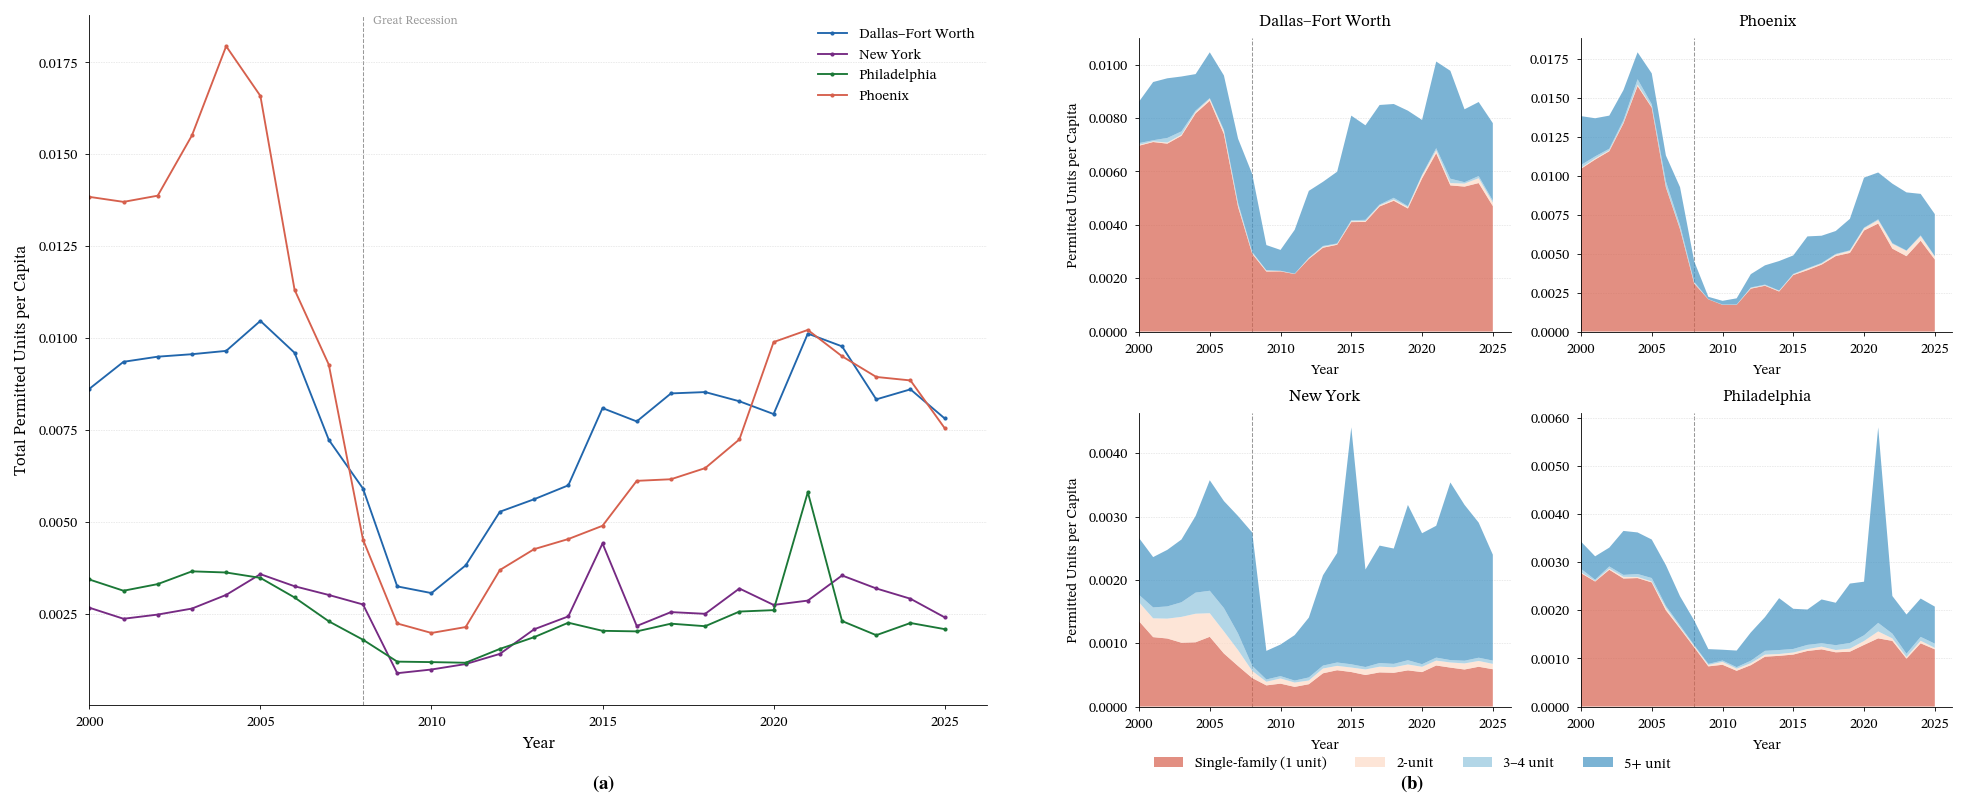
\includegraphics[width=\textwidth]{building_permits.png}
  \caption{Building permits per capita since 2000. Data derived from the US Census Building Permits Survey. A sharp decrease in building permits is seen leading up to the Great Recession and permit volume has not yet recovered. Sun Belt MSAs such as Dallas--Fort Worth--Arlington, TX and Phoenix--Mesa--Chandler, AZ outpace land-constrained MSAs like New York--Newark--Jersey City, NY-NJ and Philadelphia--Camden--Wilmington, PA-NJ-DE-MD. Building permits, with the exception of NYC, still favor single-family one-unit dwellings (red), especially in the Sun Belt MSAs. New York--Newark--Jersey City is the only MSA where multi-family dwellings take precedence over single-family ones, but Philadelphia and other northeastern cities are catching up.}
  \label{fig:building_permits}
\end{figure}

\section{UVL to Mitigate Flood Risk}
\label{sec:flood_risk}

Urban expansion and the resulting increase in impervious surfaces create a cascade of urban water-related challenges: flood risk, sewer overflow, water quality deterioration and scarcity, and extreme weather~\cite{zhang2018Urbanization}. While coastal flooding risk from sea level rise is well modeled, the rapidly increasing threat of pluvial flooding---exacerbated by urban expansion and consequent soil sealing---is often overlooked and arguably more dangerous due to its low predictability. Existing flood risk projections tend to focus on coastal cities and frequently fail to account for pluvial flooding, which is significantly increasing risk in inland cities traditionally considered safe.

The heavy rains following Hurricane Ida in New York City exemplified this vulnerability (\Cref{fig:ida_heatmap}), where sewer systems were overwhelmed by intense, rapid-onset rain, resulting in widespread structural damage across inland urban areas---a notable deviation from the coastal areas typically affected during floods in NYC. Repurposing \acrshort{uvl} is not only a promising strategy for stormwater management but in many cases a necessary one. Left unmanaged, sealed \acrshort{uvl} can worsen water quality by allowing polluted runoff to enter surrounding systems. However, when redesigned using low-impact development strategies such as rain gardens and bioswales, \acrshort{uvl} can capture, slow, and filter stormwater at the source. Repurposing \acrshort{uvl} for stormwater facilities is a viable tool to enhance climate resilience in both coastal and inland cities, particularly against pluvial flooding. That said, effectiveness depends on site-specific conditions. For example, clay-heavy soils resist infiltration, increasing the effort required to convert \acrshort{uvl} to effective stormwater infrastructure. Ultimately, the effectiveness of \acrshort{uvl} repurposing depends on both design and location. Dispersed, low-connectivity vacant parcels in highly impervious areas can reduce peak runoff and support aging infrastructure, though local conditions such as soil composition may limit performance. Overall, \acrshort{uvl} offers a flexible, distributed approach to stormwater management and improving urban flood resilience.

\begin{figure}[htbp]
  \centering
  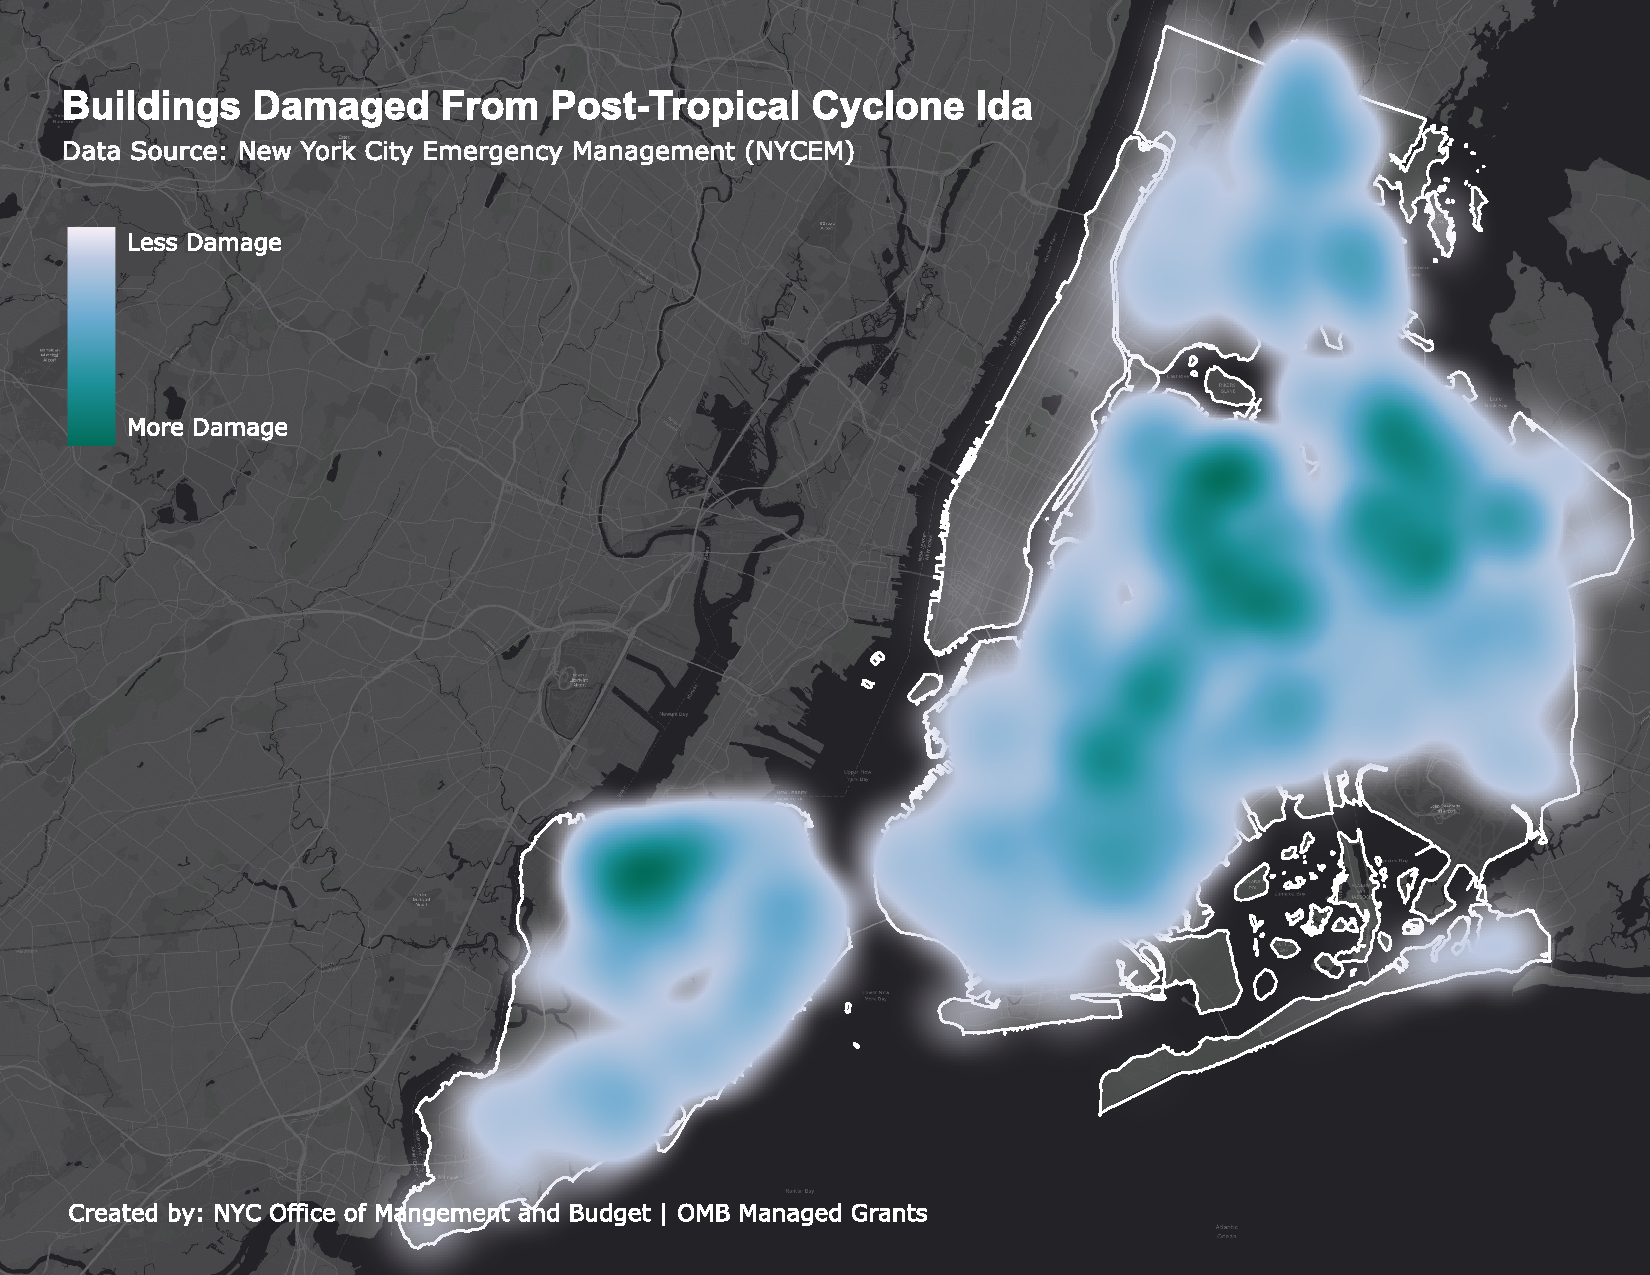
\includegraphics[width=0.85\textwidth]{DamagedBuildingsIdaHeatMap.pdf}
  \caption{Property damage from Cyclone Ida (2021), from the NYC Office of Management and Budget. While not as devastating as hurricanes Sandy and Irene, Cyclone Ida is particularly concerning as the damages were mainly from pluvial flooding due to rainfall, not coastal storm surge. Damages extended inland rather than concentrating in coastal areas---a record-breaking 3.15~inches/hour completely overwhelmed the aging sewer system designed for 1.75~in/hour.}
  \label{fig:ida_heatmap}
\end{figure}

\section{UVL for Social Good}
\label{sec:social_good}

While housing shortages and flood mitigation are two of the most urgent challenges that \acrshort{uvl} can help address, they are far from the only benefits of repurposing these spaces. \acrshort{uvl} already plays a significant social and ecological role in cities. In New York City, many vacant lots are not truly ``unused'' but instead function as community gardens, residential yards, parks, or recreational spaces~\cite{kremer2013social}. Beyond their existing uses, \acrshort{uvl} presents substantial opportunities for improving residents' wellbeing through urban greening. Converting abandoned spaces into green infrastructure---such as small urban farms or community shelters---has been shown to positively impact mental health, promote physical activity, and foster social interaction. Residents often perceive neglected vacant spaces as unsafe or unmanageable; however, their transformation into green, community-oriented areas can reduce stress, improve neighborhood perception, and strengthen social cohesion~\cite{jin2021Can}. Even in an unmanaged state, vacant lots can act as informal green spaces that support vegetation and urban wildlife, including avian species diversity~\cite{dennison2026role}. More intentional greening efforts can further enhance these ecological benefits while integrating \acrshort{uvl} into broader green infrastructure networks.

Overall, the identification and repurposing of \acrshort{uvl} offers a flexible, distributed approach to addressing both environmental and social challenges in cities. It can introduce elasticity into constrained housing markets, improve stormwater management, enhance biodiversity, and elevate quality of life. However, \acrshort{uvl} repurposing is not a one-size-fits-all solution; its success depends on careful, context-sensitive design that balances environmental goals with the needs and values of local communities.

\chapter{Background}
\label{ch:background}

\section{Previous Works}
\label{sec:previous_works}

\Acrshort{uvl} redevelopment into housing, stormwater infrastructure, or green space has demonstrated positive impacts in many case-specific studies. However, global and generalizable analyses of \acrshort{uvl} remain limited. This is largely due to the inherently heterogeneous nature of vacant land: \acrshort{uvl} varies significantly across both spatial and temporal scales, and these variations are further compounded by regional differences in urban form, governance, and land use practices.

At a fundamental level, \acrshort{uvl} is difficult to define, both semantically and physically. Broadly, it refers to urban land with little or no current functional use, yet operational definitions vary widely across the literature. \acrshort{uvl} may be defined in terms of land cover, land use, ownership, or duration of vacancy, leading to inconsistencies across studies~\cite{song2020Urban}. For example, administrative definitions such as the New York City tax code define vacant land based on the absence of ``permanent improvements,'' a criterion designed for taxation rather than spatial analysis, and one that does not translate cleanly to remote sensing or geospatial datasets~\cite{nycadmincode}.

This ambiguity is further reflected in classification schemes. Xu and Ehlers categorize vacant land into four types: brownfields, transportation-related land, natural sites, and unattended or reserve parcels~\cite{xu2022Automatica}. Their method integrates remote sensing (Sentinel-2 imagery), GIS vector layers (e.g., Urban Atlas, OpenStreetMap), and proxies for human activity such as social media data. While comprehensive, such rule-based approaches are inherently tied to local administrative definitions and data availability, limiting their transferability to other regions. In addition, key data sources---such as cadastral datasets and social media APIs---are often inaccessible, inconsistent, or paywalled, particularly in the U.S.\ and other resource-constrained contexts.

More broadly, many existing methods rely on data resolutions that are insufficient for dense urban environments. In U.S.\ cities such as New York, where vacant parcels are often small, fragmented, and embedded within dense urban fabric, coarse-resolution land cover data fails to capture meaningful patterns of vacancy. This challenge is underscored by comparative work showing that \acrshort{uvl} parcels in New York City are significantly smaller and more fragmented than those in cities such as Guangzhou, China, requiring fundamentally different identification approaches~\cite{song2020Urban}.

Recent advances in deep learning have begun to address \acrshort{uvl} detection, particularly in China. Mao et al.\ trained DeepLabv3 models across multiple regions and achieved near-human performance, but found that models trained on one region did not generalize to others, highlighting the persistent challenge of spatial generalization~\cite{mao2022Largescale}. Wang et al.\ built on this work and applied the FastSAM model to identify \acrshort{uvl} across 2,446 Chinese cities, revealing macro-scale spatial patterns~\cite{wang2026Urban}. However, these approaches adopt broader definitions of vacancy---encompassing bare land, redevelopment parcels, and edge spaces---and are designed for large, contiguous urban forms. As such, they are not well aligned with the fine-grained, parcel-level fragmentation characteristic of U.S.\ cities.

In parallel, other studies have emphasized the importance of temporal dynamics and contextual factors in understanding \acrshort{uvl}. Vacancy duration, for instance, has been shown to be a critical indicator of underlying urban processes, with longer-term vacancies associated with structural decline and higher crime rates~\cite{zhangPersistence}. Classification frameworks incorporating parcel size, ownership, and land use further demonstrate that vacancy is not a uniform condition but a spectrum of states requiring context-sensitive interpretation.

Overall, while a growing body of work has explored \acrshort{uvl} identification and classification, there remains no widely applicable, generalizable method---particularly for dense, parcel-fragmented cities such as those in the Northeast megalopolis. Existing approaches are often constrained by inconsistent definitions, limited data availability, and poor cross-regional transferability. This gap motivates the need for scalable, high-resolution, and definition-aware methods for identifying and characterizing urban vacant land.

\section{Difficulties Classifying UVL in New York City}
\label{sec:difficulties_nyc}

\begin{figure}[htbp]
  \centering
  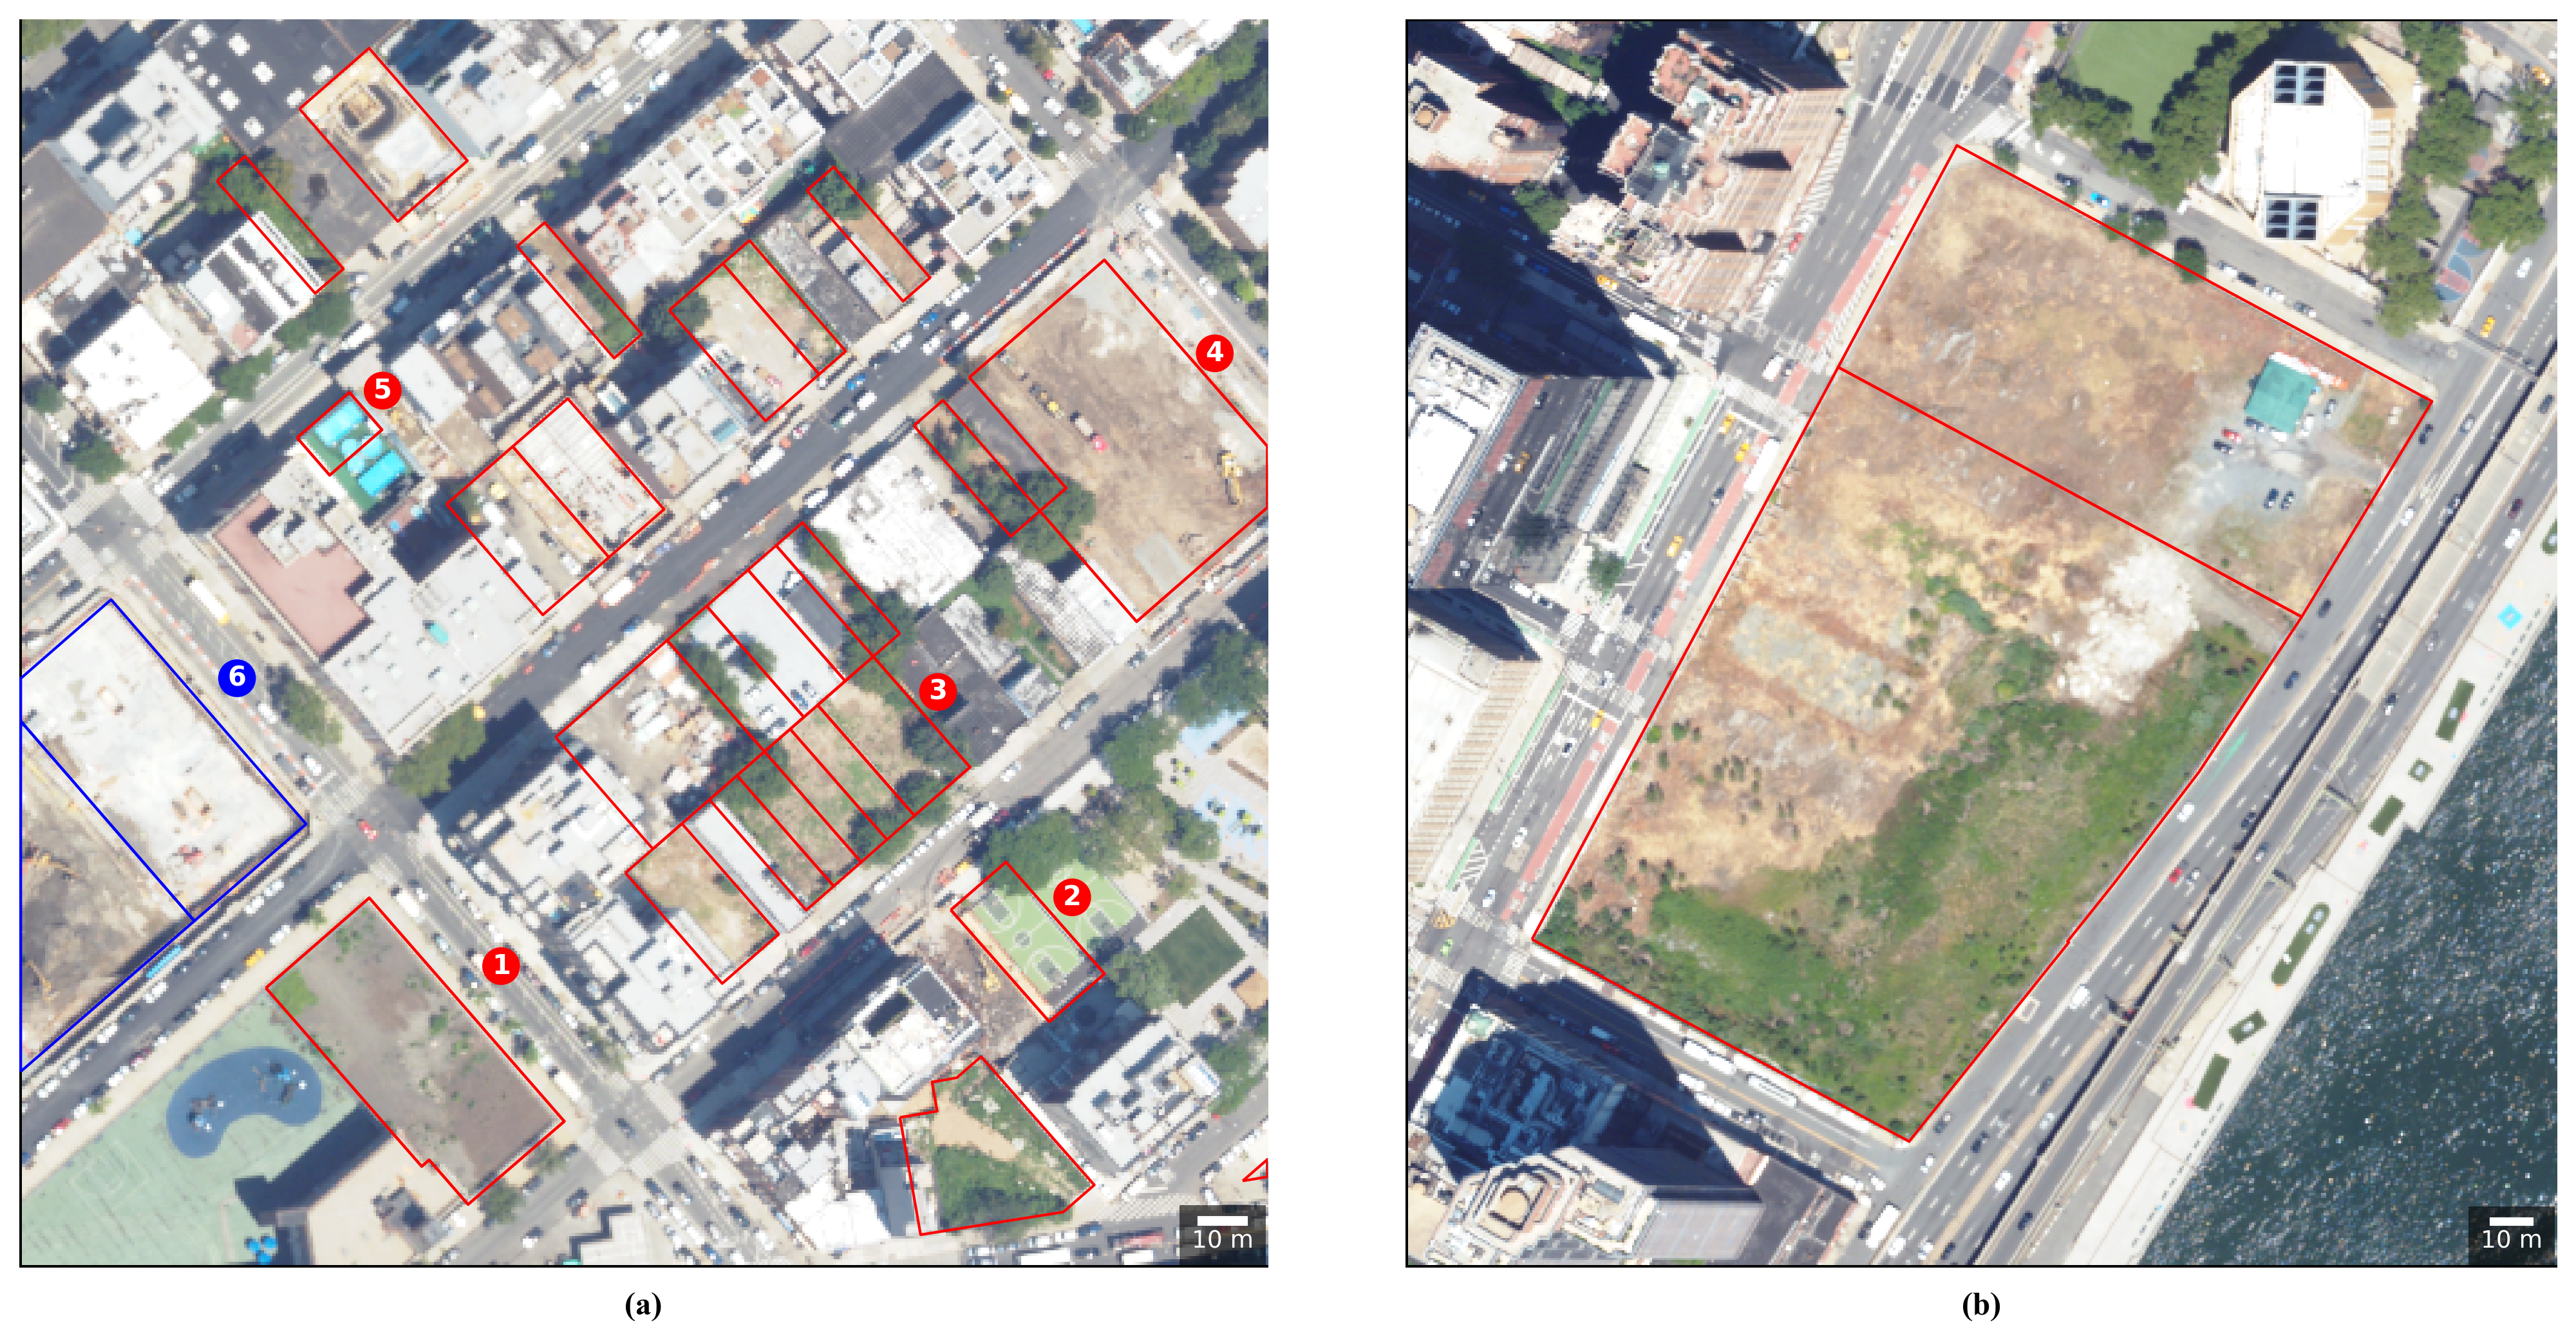
\includegraphics[width=\textwidth]{manual_inspection_of_vacant_lots.png}
  \caption{Visual inspection of parcels labeled as vacant in Williamsburg, Brooklyn. All highlighted (red) parcels are classified as vacant, while blue is non-vacant. (a)~Parcel~(1) is fully paved; (2)~is an active basketball court indistinguishable from adjacent non-vacant recreational space; (5)~appears to be a pool, suggesting functional use despite its vacant label. Parcel~(3) consists of a mix of sparse vegetation, paved areas, and informal parking. Parcels~(4) and~(6) both exhibit ongoing construction activity, yet only~(4) is labeled as vacant. These examples highlight inconsistencies in vacancy labeling, particularly during transitional states such as construction.}
  \label{fig:manual_inspection}
\end{figure}

\Cref{fig:manual_inspection} depicts the visual differences between vacant lots in Williamsburg, Brooklyn, revealing substantial heterogeneity in land use. While parcels under development may reasonably be considered vacant, there is often a lag in updating their status---evidenced by parcel~(6), where portions of exposed soil remain despite being labeled non-vacant. This underscores a key limitation of administrative vacancy datasets: they may not accurately reflect real-time land use conditions.

NYC's MapPLUTO dataset is used here for labels and discussed further in \Cref{sec:mappluto}, but a preliminary analysis on different land cover over \acrshort{uvl} was conducted to exemplify their high variance.

\begin{figure}[htbp]
  \centering
  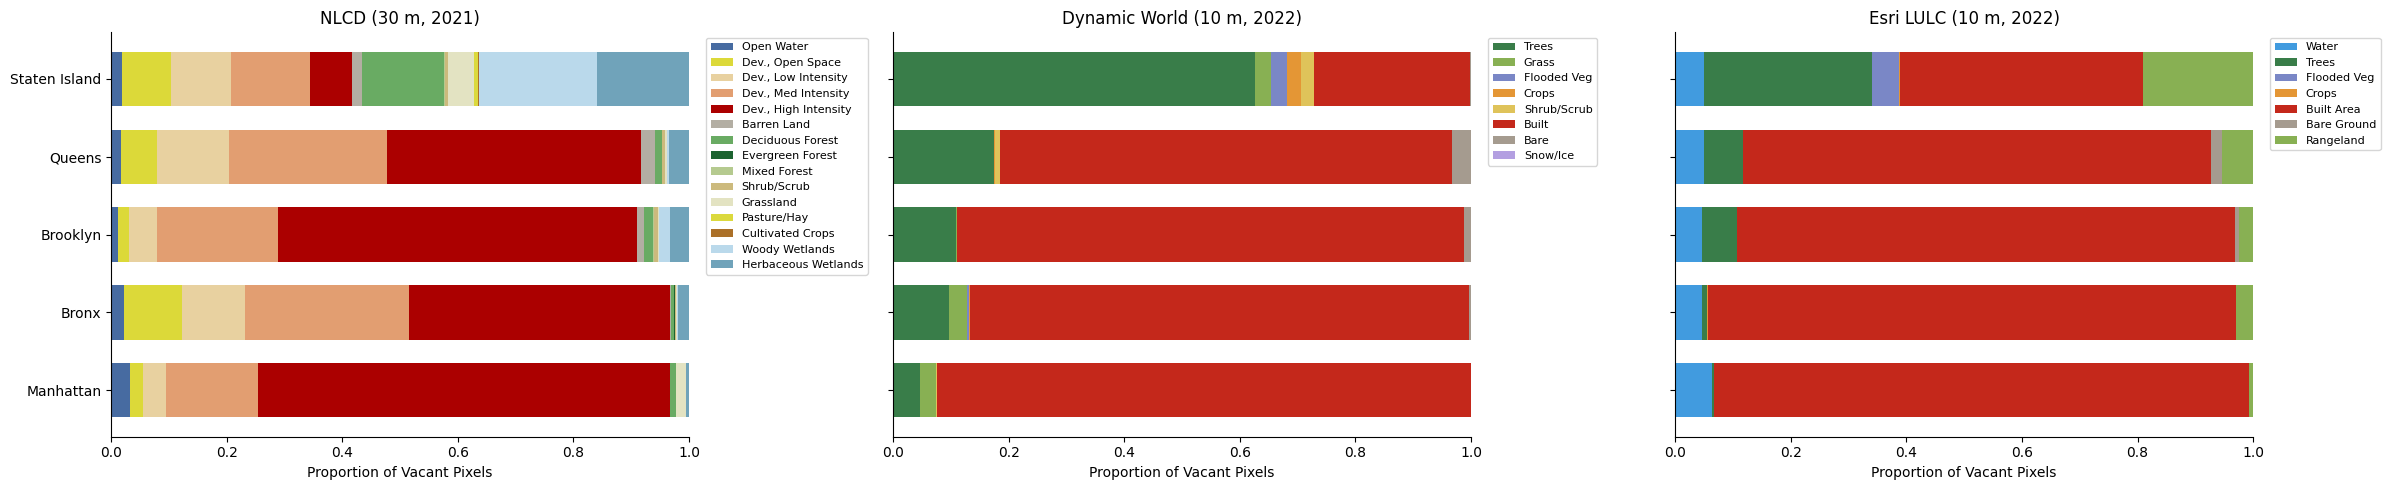
\includegraphics[width=\textwidth]{lulc_vacant.png}
  \caption{Land use and land cover distribution across vacant lots by borough. Within each borough, there is a varied amount of land cover classes.}
  \label{fig:lulc_vacant}
\end{figure}

\chapter{Data}
\label{ch:data}

\section{Data Sources}
\label{sec:data_sources}

As per the open-source requirement chosen for this study, all data sources used are open source or reproducible through open-source methods.

\subsection{NAIP Imagery}
\label{sec:naip}

The \acrfull{naip}, administered by the USDA, has acquired high-resolution aerial orthophotos across the continental United States since 2003. Originally capturing imagery at 1~m resolution on a five-year revisit cycle per state, the program transitioned to a three-year cycle in 2009. Near-infrared was piloted in Arizona in 2007 and became a default four-band product (Red, Green, Blue, \acrshort{nir}) in 2010. In 2018, the native spatial resolution was upgraded to 0.6~m per pixel, with 0.3~m available for some coastal states. Imagery is orthorectified to a horizontal accuracy of 4~meters at 95\% confidence, referenced to NAD83, and distributed as quarter-quadrangle tiles ($3.75'$ longitude $\times$ $3.75'$\ latitude with a 300-meter buffer). Cloud cover is limited to at most 10\% per tile.

\acrshort{naip} is freely available through providers such as Google Earth Engine, AWS STAC APIs, and the USGS data portal. For this study, 2022 NYC tiles were downloaded from the Microsoft Planetary Computer STAC API at no cost. NYC was imaged across three acquisition dates in 2022: July~19 (17 center tiles), September~15 (24 tiles covering the outer boroughs), and October~7 (6 tiles covering southwest Staten Island). Of the 85 quarter-quadrangle tiles downloaded, 38 covering New Jersey border areas were excluded. The remaining 47 tiles were mosaicked into a single virtual raster (VRT) using GDAL, with later acquisition dates placed on top to resolve any overlap. All bands were normalized to $[0,\,1]$ prior to model input. The 2022 acquisition year was chosen to align temporally with the MapPLUTO 22v3 parcel dataset.

Despite its utility as a freely available, high-resolution national dataset, \acrshort{naip} has notable limitations relevant to this study. Because imagery acquisition is partially state-funded, spatial resolution and spectral options (e.g., 0.3~m) vary by state, limiting portability of methods to other regions. The program does not guarantee annual coverage. Perhaps most practically, there is a substantial lag between imagery acquisition and availability on easy-to-use APIs: as of writing, 2024 imagery is not available on Planetary Computer or GEE and requires navigating USDA/USGS government portals directly. This lag constrains how current a deployed model's inputs can be relative to administrative records.

\subsection{NYC MapPLUTO}
\label{sec:mappluto}

MapPLUTO (Map Primary Land Use Tax Lot Output) is a publicly available geospatial dataset released quarterly by New York City's Department of City Planning that merges tax lot boundaries with land use, zoning, and building information for every parcel in the city. Vacancy is encoded by Building Class codes V0 through V9 (vacant land subtypes) and G7 (unlicensed parking lots). Of the 856,998 parcels in MapPLUTO 22v3, 30,792 (3.6\%) carry a vacant Building Class code. Parcel geometries are natively in EPSG:2263 (New York State Plane) and were reprojected to EPSG:26918 (UTM Zone 18N) to align with the \acrshort{naip} raster grid.

\subsection{NYC DoITT Planimetric Database}
\label{sec:doitt}

The NYC Department of Information Technology and Telecommunications (DoITT) Planimetric Database is a citywide vector dataset derived from aerial photogrammetry, capturing physical features of the urban environment as mapped polygons. For this study, the \texttt{ROADBED} layer of 104,959 MultiPolygon features representing the actual paved surface of every road was used to mask road surfaces in the vacancy mask (\Cref{sec:vacancy_mask}). The motivation is that road surfaces within parcel boundaries are a significant source of label noise: many parcels classified as vacant by MapPLUTO are highway shoulders, elevated highway footprints, or DOT-owned road infrastructure where the visible surface is entirely asphalt. Burning these surfaces to ignore (255) prevents the model from learning an association between road asphalt and vacancy. While this dataset is specific to NYC, it is not considered out of line with the open-source requirement, as many open-source datasets for road masking exist elsewhere (e.g., OSM centerlines with a buffer).

\section{Labels and Vacancy Mask}
\label{sec:vacancy_mask}

\subsection{Vacancy Mask Construction}

Ground truth labels are encoded as a binary vacancy mask produced by rasterizing MapPLUTO parcel boundaries onto the \acrshort{naip} pixel grid at 0.6~m resolution. The mask uses three values: 0~(non-vacant), 1~(vacant), and 255~(ignore). Pixels assigned 255 are excluded from both loss computation during training and metric computation during evaluation~\cite{everingham2010pascal}. Beyond handling label ambiguity, the ignore class also serves a class-imbalance purpose: masking out roads, water, and other surfaces where vacancy is structurally impossible prevents hundreds of millions of additional non-vacant pixels from diluting an already sparse 3.4\% vacancy signal.

The mask was produced through two successive versions. An initial mask (v1) was used for early training runs; systematic inspection of model predictions identified label errors that were corrected in a refined mask (v2), which was used for all final reported results. The pipeline steps are as follows:

\begin{enumerate}
  \item \textbf{Base burn:} All MapPLUTO parcel polygons were rasterized to 0 (non-vacant). Pixels falling outside any parcel boundary---roads, water bodies, and other unregistered land---receive no label and default to 255 (ignore).

  \item \textbf{Vacant burn:} Parcels with vacant Building Class codes (V0--V9, G7) are overwritten with 1 (vacant). Vacant parcels smaller than 50~pixels ($\sim$18~m\textsuperscript{2}) were set to 255, as they are considered too small for meaningful spectral characterization at 0.6~m resolution.

  \item \textbf{Manual corrections:} A small set of parcels were reassigned based on visual inspection of \acrshort{naip} imagery and, for v2, cross-referencing a newer MapPLUTO vintage (23v2) as well as analyzing initial model runs. The v2 modifications include parcels under active construction, waterfront parcels extending into water, parcels obstructed by elevated highways, and DOT-owned highway shoulders mislabeled as vacant. Rikers Island was set to ignore given its anomalous land use as a detention facility and its proximity to both Bronx and Queens, which is important for the spatial split (see \Cref{sec:borough_split}). A detailed list of manual corrections is provided in \Cref{appendix:manual_corrections}.

  \begin{table}[H]
    \centering
    \caption{Summary of manual mask corrections between v1 and v2.}
    \label{tab:mask_corrections}
    \begin{tabular}{lcc}
      \toprule
      \textbf{Action} & \textbf{v1} & \textbf{v2} \\
      \midrule
      Set to ignore (255)  & Shadow-occluded + South Brother Island & $\sim$49 total \\
      Forced non-vacant (0) & --- & 11 (buildings present; highway parcels) \\
      Forced vacant (1) & --- & 7 (visual confirmation or vintage cross-check) \\
      \bottomrule
    \end{tabular}
  \end{table}

  \item \textbf{Boundary erosion:} A 2-pixel morphological erosion is applied at transitions between vacant and non-vacant parcels to reduce improper labeling due to relief displacement artifacts from orthoimagery. The transition zone is identified by dilating both classes and computing their overlap; pixels in this overlap zone on the vacant side are set to 255. This reduces noise from imprecise parcel boundary rasterization and mixed pixels at parcel edges. Boundaries between two parcels of the same class are left untouched.

  \item \textbf{Road masking:} In v1, road masking was not augmented intentionally, as most MapPLUTO parcels do not contain roads. After initial runs revealed the need to explicitly mask roads (elevated highway obstruction, roads within vacant parcels), the v2 mask incorporated the NYC DoITT Planimetric Database roadbed polygons, burned into the raster as 255 (ignore).
\end{enumerate}

\begin{figure}[htbp]
  \centering
  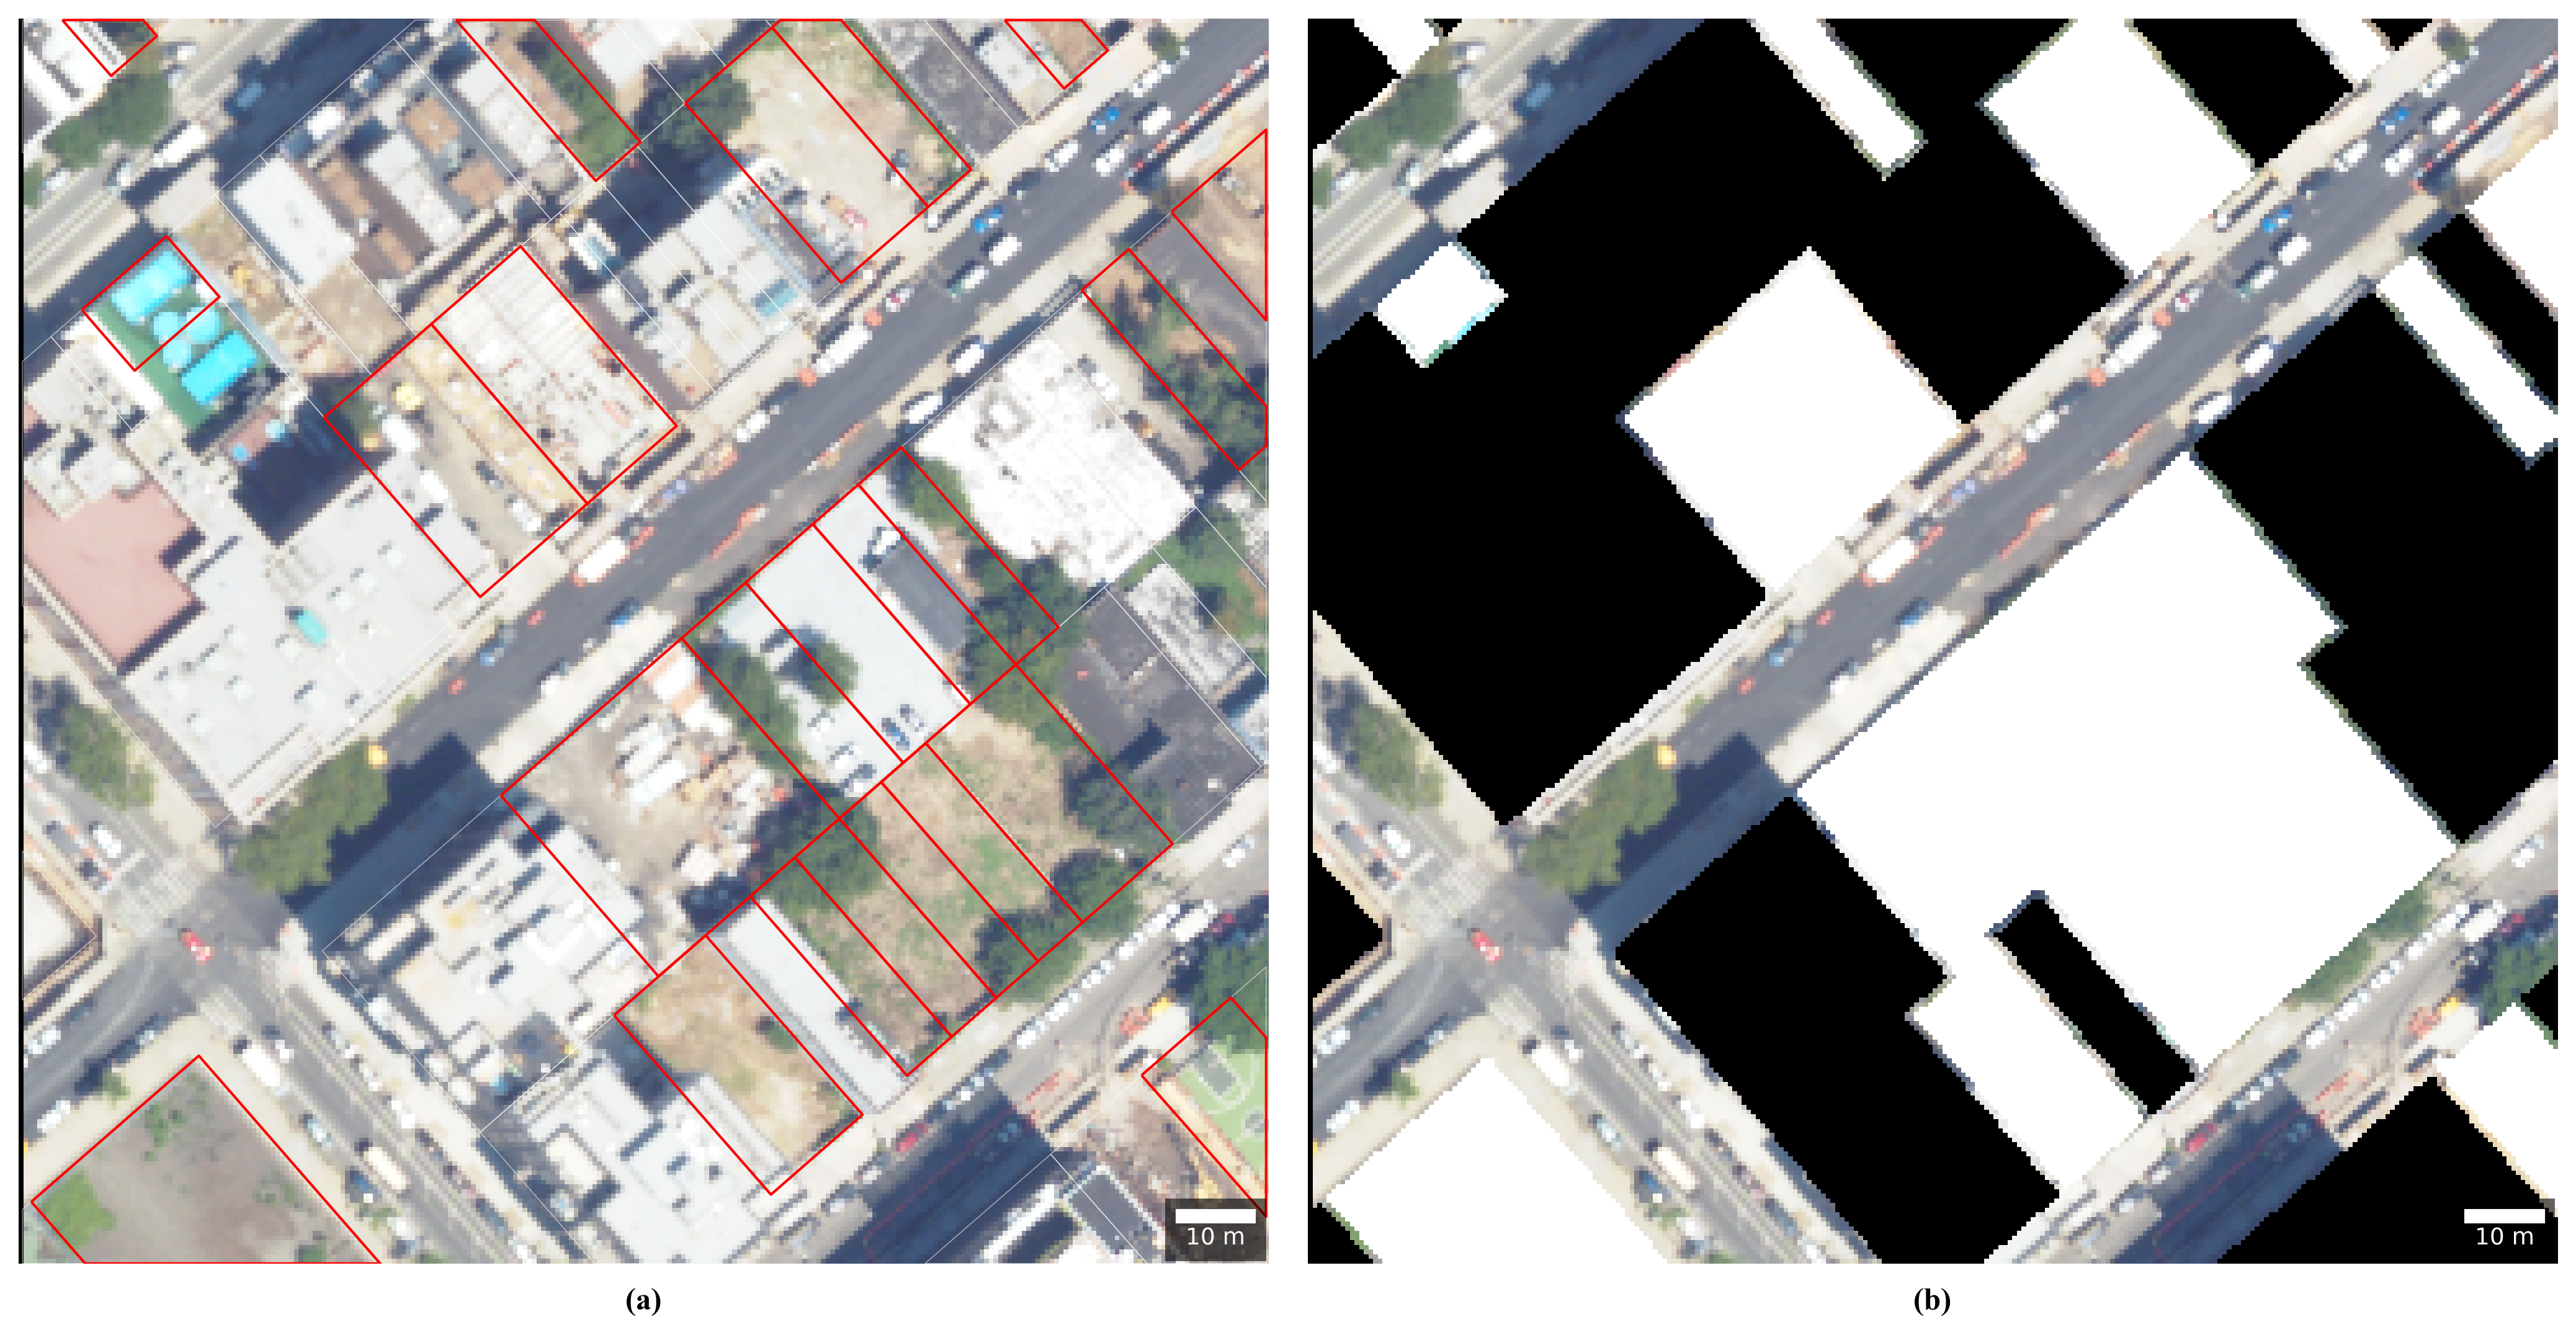
\includegraphics[width=0.85\textwidth]{sample_vacancy_mask.png}
  \caption{Sample of the vacancy mask. White pixels are vacant (1), black are non-vacant (0), and areas without a parcel are ignore (255). Boundaries between vacant and non-vacant parcels were dilated to reduce noisy signal from shadows or relief distortion.}
  \label{fig:vacancy_mask}
\end{figure}

\subsection{v1 vs.\ v2 Masks}

After the v1 pipeline, the mask contained 29,336 vacant parcels (3.4\% of 855,322 eligible parcels). The v2 corrections reduced vacant pixel counts in every borough, with Queens seeing the largest change due to the planimetric roadbed mask converting 1.39M previously vacant road pixels to ignore (255).

\begin{table}[htbp]
  \centering
  \caption{Pixel changes from vacancy mask v1 to v2.}
  \label{tab:v1_v2_changes}
  \begin{tabular}{lrr}
    \toprule
    \textbf{Borough} & \textbf{Vacant pixel $\Delta$} & \textbf{Ignore pixel $\Delta$} \\
    \midrule
    Manhattan     & $-296{,}000$   & $+4{,}700{,}000$ \\
    Bronx         & $-296{,}000$   & $+11{,}100{,}000$ \\
    Brooklyn      & $-385{,}000$   & $+9{,}500{,}000$ \\
    Queens        & $-1{,}390{,}000$ & $+41{,}400{,}000$ \\
    Staten Island & $-2{,}150{,}000$ & $+9{,}800{,}000$ \\
    \bottomrule
  \end{tabular}
\end{table}

\subsection{Label Noise}

Several sources of label noise are inherent to the use of administrative vacancy designations as ground truth for an image segmentation task:

\paragraph{Temporal Lag.} Building Class codes are updated manually on an irregular schedule. Parcels under active construction may retain a vacant label until a foundation is in place; recently demolished lots may not yet be reclassified as vacant. Both directions of lag are visible in the 2022 imagery---construction sites with bare soil labeled vacant, and recently cleared lots still labeled non-vacant.

\paragraph{Administrative vs.\ Visual Mismatch.} The most fundamental noise source is that administrative vacancy is not a visual property. Two parcels can be spectrally identical yet carry opposite labels (see \Cref{fig:manual_inspection}). A well-maintained grassy lot and an overgrown abandoned lot may both be classified as vacant, while a visually similar grassy lot that is part of a park is classified as non-vacant. Similarly, a parking lot with organized vehicles may be non-vacant while an identical-looking lot without a permanent structure may be vacant. These cases represent an irreducible noise floor that limits the maximum achievable performance of any vision-based model. The qualitative analysis in \Cref{sec:qualitative} provides a detailed taxonomy of these failure modes.

\paragraph{Shadow Occlusion.} In dense urban environments, tall buildings cast shadows that obscure ground-level features in aerial imagery. Nine parcels fully occluded by shadow were manually identified and excluded. However, partial shadow effects along building edges remain a source of noise, particularly in Manhattan (which was excluded from the study for this reason).

\section{Borough-Based Spatial Split}
\label{sec:borough_split}

To prevent geographic leakage between training and evaluation, the dataset is split spatially by borough rather than by random sampling of patches. NYC's five boroughs exhibit distinct urban morphologies---lot sizes, building density, vegetation patterns, and land use mixtures vary substantially across boroughs---making this a meaningful test of spatial generalization.

\begin{table}[htbp]
  \centering
  \caption{Borough-based spatial split.}
  \label{tab:borough_split}
  \begin{tabular}{lcll}
    \toprule
    \textbf{Borough} & \textbf{BoroCode} & \textbf{Split} & \textbf{Rationale} \\
    \midrule
    Queens         & 4 & Train    & Largest number of vacant pixels; diverse lot types \\
    Bronx          & 2 & Val      & Distinct urban morphology from training borough \\
    Brooklyn       & 3 & Test     & Good distribution of vacancy types \\
    Manhattan      & 1 & Excluded & Tall building occlusion renders imagery unreliable \\
    Staten Island  & 5 & Excluded & Overwhelmingly tree cover; atypical of dense urban fabric \\
    \bottomrule
  \end{tabular}
\end{table}

\section{Patch Extraction}
\label{sec:patch_extraction}

Remote sensing imagery is too large to process directly with convolutional neural networks and must be divided into smaller patches for training and inference~\cite{huang2019Tiling}. Patches of $512\times512$ and $1024\times1024$ pixels were evaluated (corresponding to approximately 307~m and 614~m spatial extent at 0.6~m resolution). Patches are extracted on a non-overlapping grid (stride equal to patch size) to prevent data leakage between patches during training. A patch is retained if at least 50\% of its pixels carry a label (0 or 1 rather than 255), ensuring patches are not dominated by roads or water. Any patch containing at least one vacant pixel is also retained regardless of the 50\% threshold.

At $512\times512$ patch size, this yields:

\begin{table}[htbp]
  \centering
  \caption{Patch extraction statistics at $512\times512$ pixels.}
  \label{tab:patch_stats}
  \begin{tabular}{lrrrr}
    \toprule
    \textbf{Split} & \textbf{Patches} & \textbf{Vacant Pixels} & \textbf{Non-Vacant Pixels} & \textbf{Vacant \%} \\
    \midrule
    Train (Queens)    & 12,576 & 19,729,417 & 566,361,850  & 3.37\% \\
    Val (Bronx)       &  8,137 & 10,877,486 & 352,131,274  & 3.00\% \\
    Test (Brooklyn)   &  4,943 &  8,390,527 & 216,060,926  & 3.74\% \\
    \bottomrule
  \end{tabular}
\end{table}

The severe class imbalance ($\sim$3.4\% vacant pixels) is addressed through oversampling and loss function weighting, described in \Cref{sec:class_imbalance}.

During inference, a smaller stride (e.g., 256 for 512-patch, 512 for 1024-patch) is used to produce overlapping predictions that are averaged, reducing edge artifacts from patch boundaries.

\section{CRS Alignment}
\label{sec:crs}

All geospatial data was reprojected to EPSG:26918 (UTM Zone 18N), the native \acrshort{crs} of the \acrshort{naip} imagery. MapPLUTO parcels (originally EPSG:2263, New York State Plane) and NYC Planimetric roadbed polygons were reprojected to match the \acrshort{naip} raster grid prior to rasterization. Borough boundaries from TIGER county shapefiles were similarly aligned.

\chapter{Methods}
\label{ch:methods}

\section{Problem Formulation}
\label{sec:problem}

The task is formulated as binary semantic segmentation: given a multi-band aerial image patch, assign each pixel a label of vacant (1) or non-vacant (0).

Pixel-level segmentation was chosen over parcel-level classification because pixel-level models do not require parcel boundary data at inference time. Parcel data, managed at the county or local level, is prone to errors in land use classification, temporal resolution, and boundary delineation, especially in smaller cities with limited assessor resources where \acrshort{uvl} repurposing could have disproportionate value. Furthermore, even in smaller jurisdictions that do have digitized cadastral data, it is often paywalled. A model that operates on imagery alone can be deployed anywhere \acrshort{naip} coverage exists, generating a shortlist of potentially vacant areas for human review without requiring cadastral data.

\section{Evaluation Metrics}
\label{sec:metrics}

The severe class imbalance, the rarity of the positive class, and the irreducible label noise due to differing administrative and spatial definitions of vacancy motivate the following ranking of metrics.

The generalized $F_\beta$ score takes the harmonic mean of precision and recall, with $\beta$ controlling the relative weight:

\begin{equation}
  F_\beta = (1 + \beta^2) \cdot \frac{\text{precision} \cdot \text{recall}}{\beta^2 \cdot \text{precision} + \text{recall}}
  \label{eq:fbeta}
\end{equation}

With $\beta = 1$, the $F_1$ score is retrieved, assigning equal weight to both precision and recall. With $\beta = 2$, the $F_2$ score places four times the weight on recall. As $\beta$ increases, the model is rewarded more for missing fewer positives, even at the cost of precision.

\paragraph{F2 Score (Primary Metric).}
The $F_2$ score weighs recall 4$\times$ heavier than precision:

\begin{equation}
  F_2 = 5 \cdot \frac{\text{precision} \cdot \text{recall}}{4 \cdot \text{precision} + \text{recall}}
  \label{eq:f2}
\end{equation}

In a screening application, a false negative---a vacant lot the model misses entirely---is costlier than a false positive that a human reviewer can quickly discard. With only 3.4\% of labeled pixels being vacant, even a model with moderate recall will generate manageable false positive volumes relative to the total parcel count. $F_2$ encodes this asymmetry directly. Accuracy is not reported: a model predicting all pixels as non-vacant would achieve $\sim$97\% accuracy, making the metric uninformative for this task.

\paragraph{F1 Score.}
$F_1$ is reported as a secondary metric. It treats precision and recall symmetrically and is equivalent to the Dice coefficient, providing a reference point against studies that may prioritize $F_1$.

\paragraph{Average Precision (AP).}
Average precision is the area under the precision--recall curve across all thresholds. It is analogous to AUC in a balanced binary classification problem.

\paragraph{Intersection over Union (IoU).}
\acrshort{iou} is reported for completeness and cross-paper comparability:

\begin{equation}
  \text{IoU} = \frac{TP}{TP + FP + FN}
  \label{eq:iou}
\end{equation}

\acrshort{iou} is a stricter metric than $F_1$---it is more sensitive to false positives---and is the standard in general semantic segmentation benchmarks. However, it penalizes recall and precision equally, which is not well-aligned with the recall-priority framing of this task. \acrshort{iou} is reported but not used for model selection.

Note that some prior works (e.g., Mao et al., 2022) compute \acrshort{iou} after dilating predicted polygons to account for boundary uncertainty. This study reports pixel-level \acrshort{iou} without dilation, which is a stricter measure and not directly comparable to those results.

Additional metrics reported for diagnostic value include precision, recall, and Cohen's $\kappa$.

\paragraph{Pixel-Level vs.\ Parcel-Level Metrics.}
All metrics in this study are computed at the pixel level. In jurisdictions with parcel data, a parcel-level evaluation---``what fraction of vacant tax lots were flagged?''---would be more operationally relevant, as a planner cares about lots, not individual pixels. Pixel-level metrics are biased toward large lots: a single correctly detected 10,000-pixel parcel contributes more to aggregate $F_2$ than many small 200-pixel parcels that were missed. However, the model is designed to operate in jurisdictions that lack digitized parcel boundaries, where pixel-level metrics are the only evaluation possible.

\paragraph{Loss--Metric Alignment.}
No standard differentiable surrogate exists for $F_2$. The training loss (\acrshort{bce} + Lov\'{a}sz-hinge) directly optimizes a proxy for \acrshort{iou}, not $F_2$. The recall bias needed for strong $F_2$ performance is instead induced indirectly through \texttt{pos\_weight=30} in the \acrshort{bce} term, which amplifies the gradient contribution of positive pixels and pushes the learned decision boundary toward higher recall. This indirect approach is a known limitation: the model optimizes one objective during training and is evaluated on another.

\paragraph{Threshold Selection.}
All models output per-pixel probabilities. A threshold sweep from 0.01 to 0.99 is performed on the validation set; thresholds maximizing $F_2$ and $F_1$ are identified separately. Unless otherwise noted, reported metrics use the $F_2$-optimal validation threshold.

\section{Input Features and Feature Engineering}
\label{sec:features}

The primary input to all models is the four-band \acrshort{naip} patch (R, G, B, \acrshort{nir}), normalized to $[0,\,1]$, and an optional building segmentation probability map. Early runs added eight spectral features based on EDA (see \Cref{appendix:spectral_signal}), with the intention of accelerating convergence, but these had no notable impact and added noise.

\subsection{Building Segmentation}
\label{sec:building_seg}

A building segmentation mask was generated with the open-source UAGLNet model from Hugging Face, a pre-trained U-Net with a ResNet-34 backbone. Using this model, inference was performed on the RGB bands of the \acrshort{naip} mosaic. The motivation is that building presence is a strong negative indicator of vacancy: a pixel confidently classified as rooftop cannot be vacant land. This auxiliary channel may reduce false positives on building surfaces and resolve ambiguity between bare soil and impervious rooftop materials, which share similar RGBN signatures.

Rather than using a provided dataset of building footprints (e.g., Microsoft Planetary Computer's building footprints or NYC building footprints), inference was performed on the \acrshort{naip} imagery for two reasons: (1)~to eliminate any temporal lag between \acrshort{naip} and building footprint acquisition, and (2)~to maintain an open-source pipeline, as many cities may not have up-to-date, available building footprint data.

Experiments compared 4-channel (RGBN only) and 5-channel (RGBN + building probability) inputs. Results and ablation are in \Cref{sec:results_overview}.

\section{Models}
\label{sec:models}

Preliminary pixel-level baselines (Random Forest, LightGBM) trained without spatial context performed poorly, confirming that neighboring pixel relationships and texture are essential for this segmentation task (see \Cref{appendix:tree_baselines}). Two convolutional architectures were selected for this work: U-Net and DeepLabV3+.

The U-Net architecture (Ronneberger et al., 2015) pairs a contracting encoder with an expanding decoder, connected by skip connections at every layer that preserve spatial detail lost during downsampling (\Cref{fig:unet_arch}). Its parameter efficiency and strong performance with limited training data have made it a standard for biomedical image segmentation, where detecting rare structures is common---properties well-suited to \acrshort{uvl} detection, where the positive class comprises only 3.4\% of labeled pixels.

\begin{figure}[htbp]
  \centering
  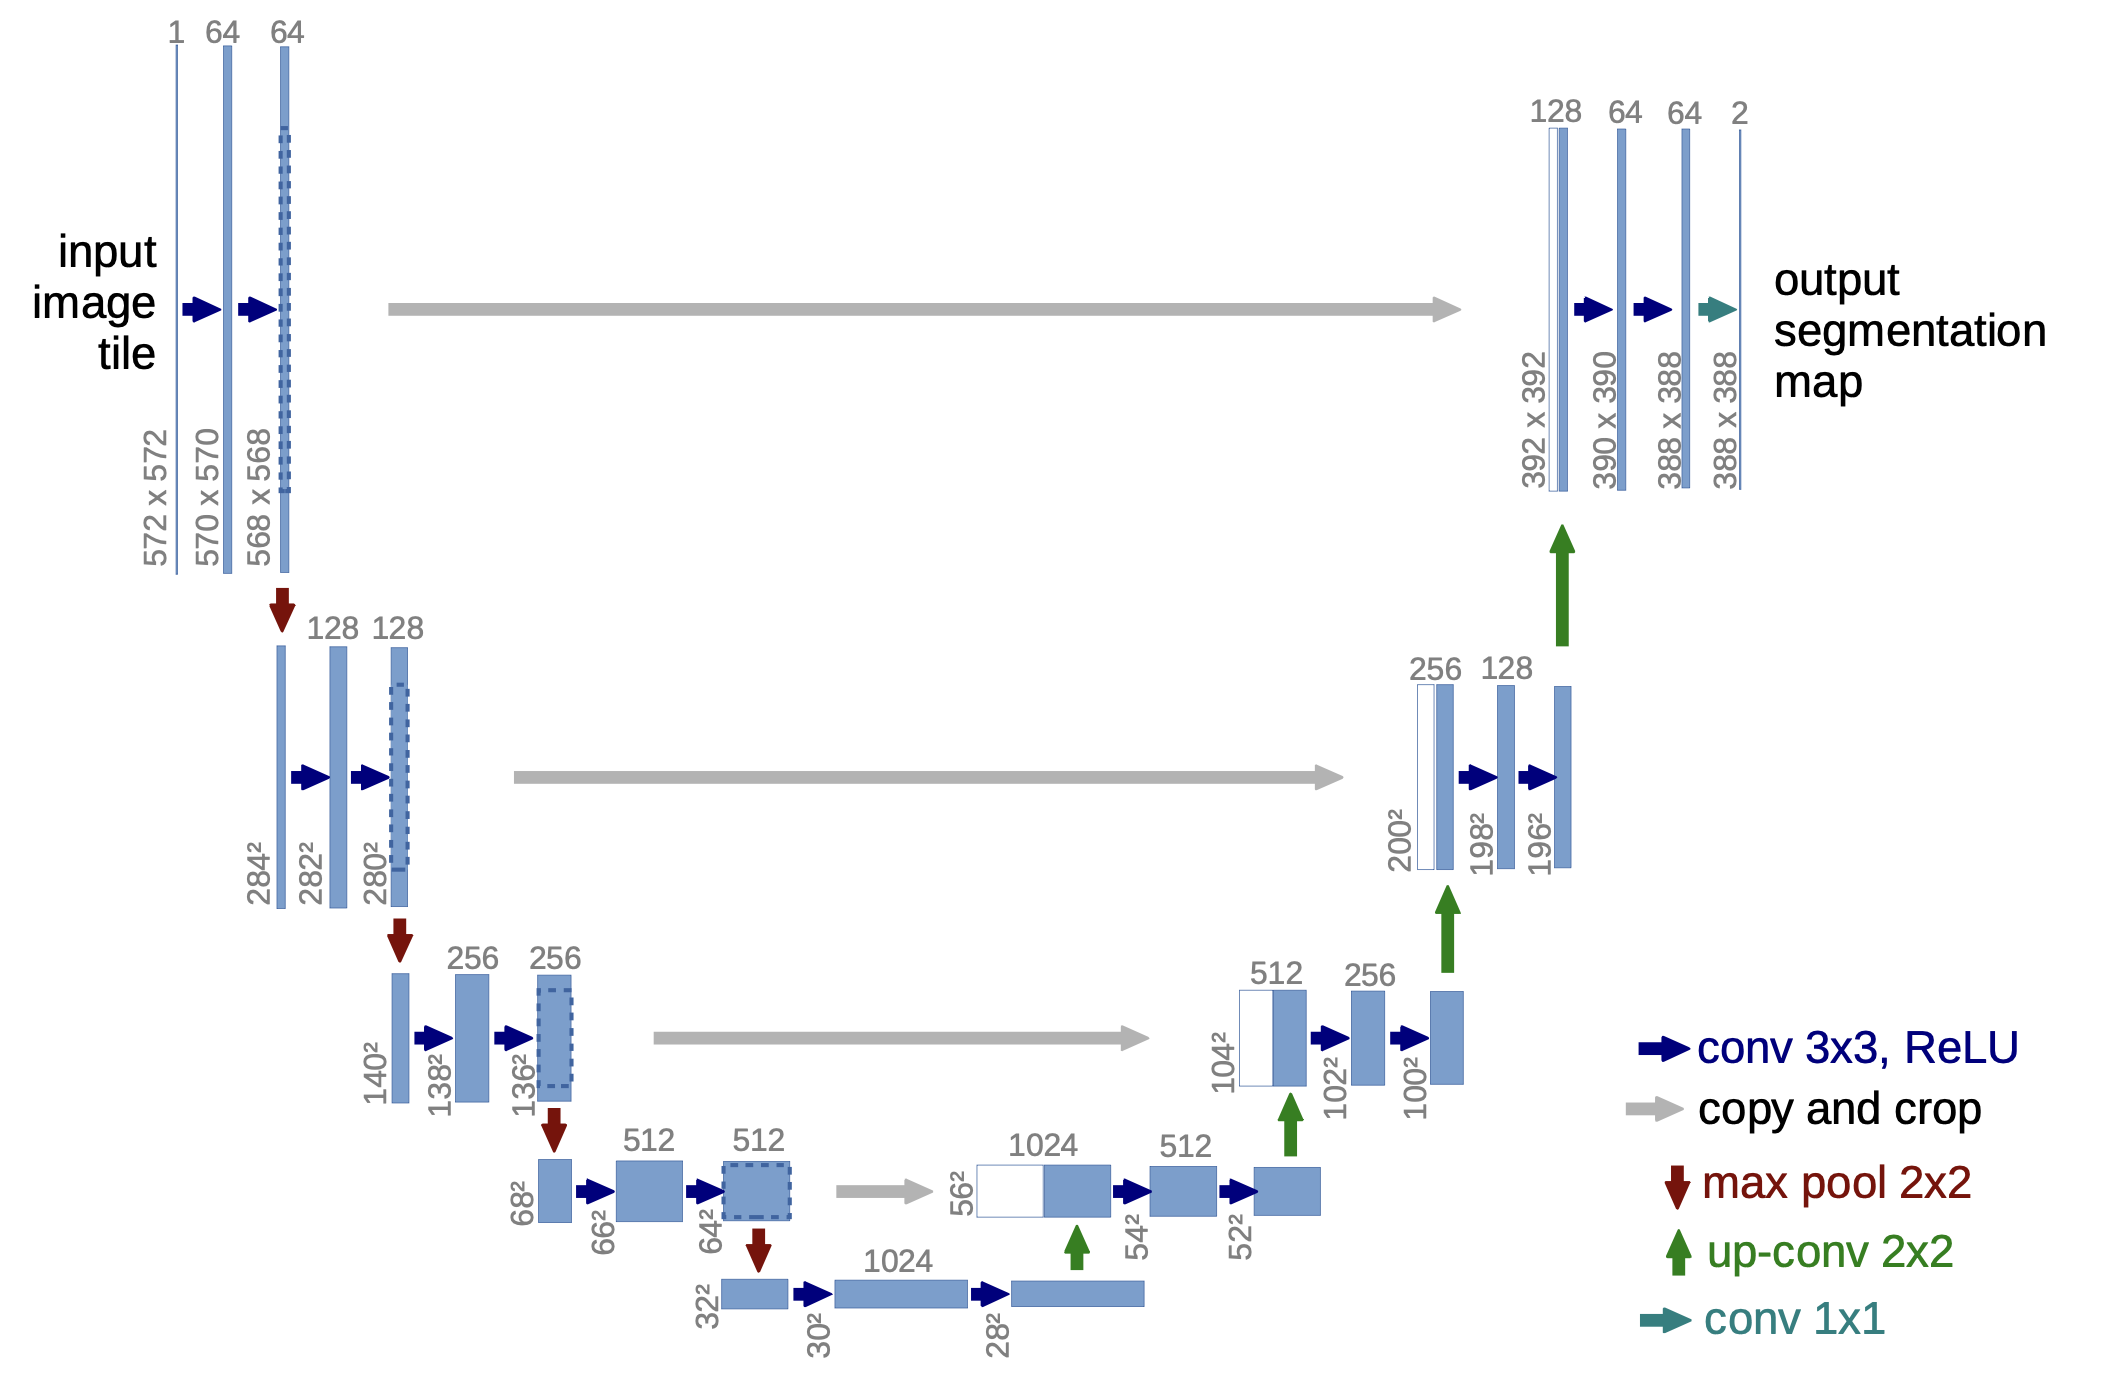
\includegraphics[width=\textwidth]{unet_ronneberger.png}
  \caption{U-Net architecture from Ronneberger et al.\ (shown here with 64 feature channels and a $32\times32$ lowest-resolution representation). The left side of the ``U'' is the encoder, progressively reducing spatial resolution while learning higher-level features, and the right side is the decoder, which restores spatial resolution for precise localization. Gray arrows indicate skip connections that pass high-resolution feature maps from the encoder to the decoder, preserving fine spatial detail.}
  \label{fig:unet_arch}
\end{figure}

DeepLabV3 (Chen et al., 2017) captures multi-scale context through \acrfull{aspp}, which applies parallel dilated convolutions at multiple rates, allowing the model to simultaneously capture both local and global spatial patterns (\Cref{fig:atrous_conv}).

\begin{figure}[htbp]
  \centering
  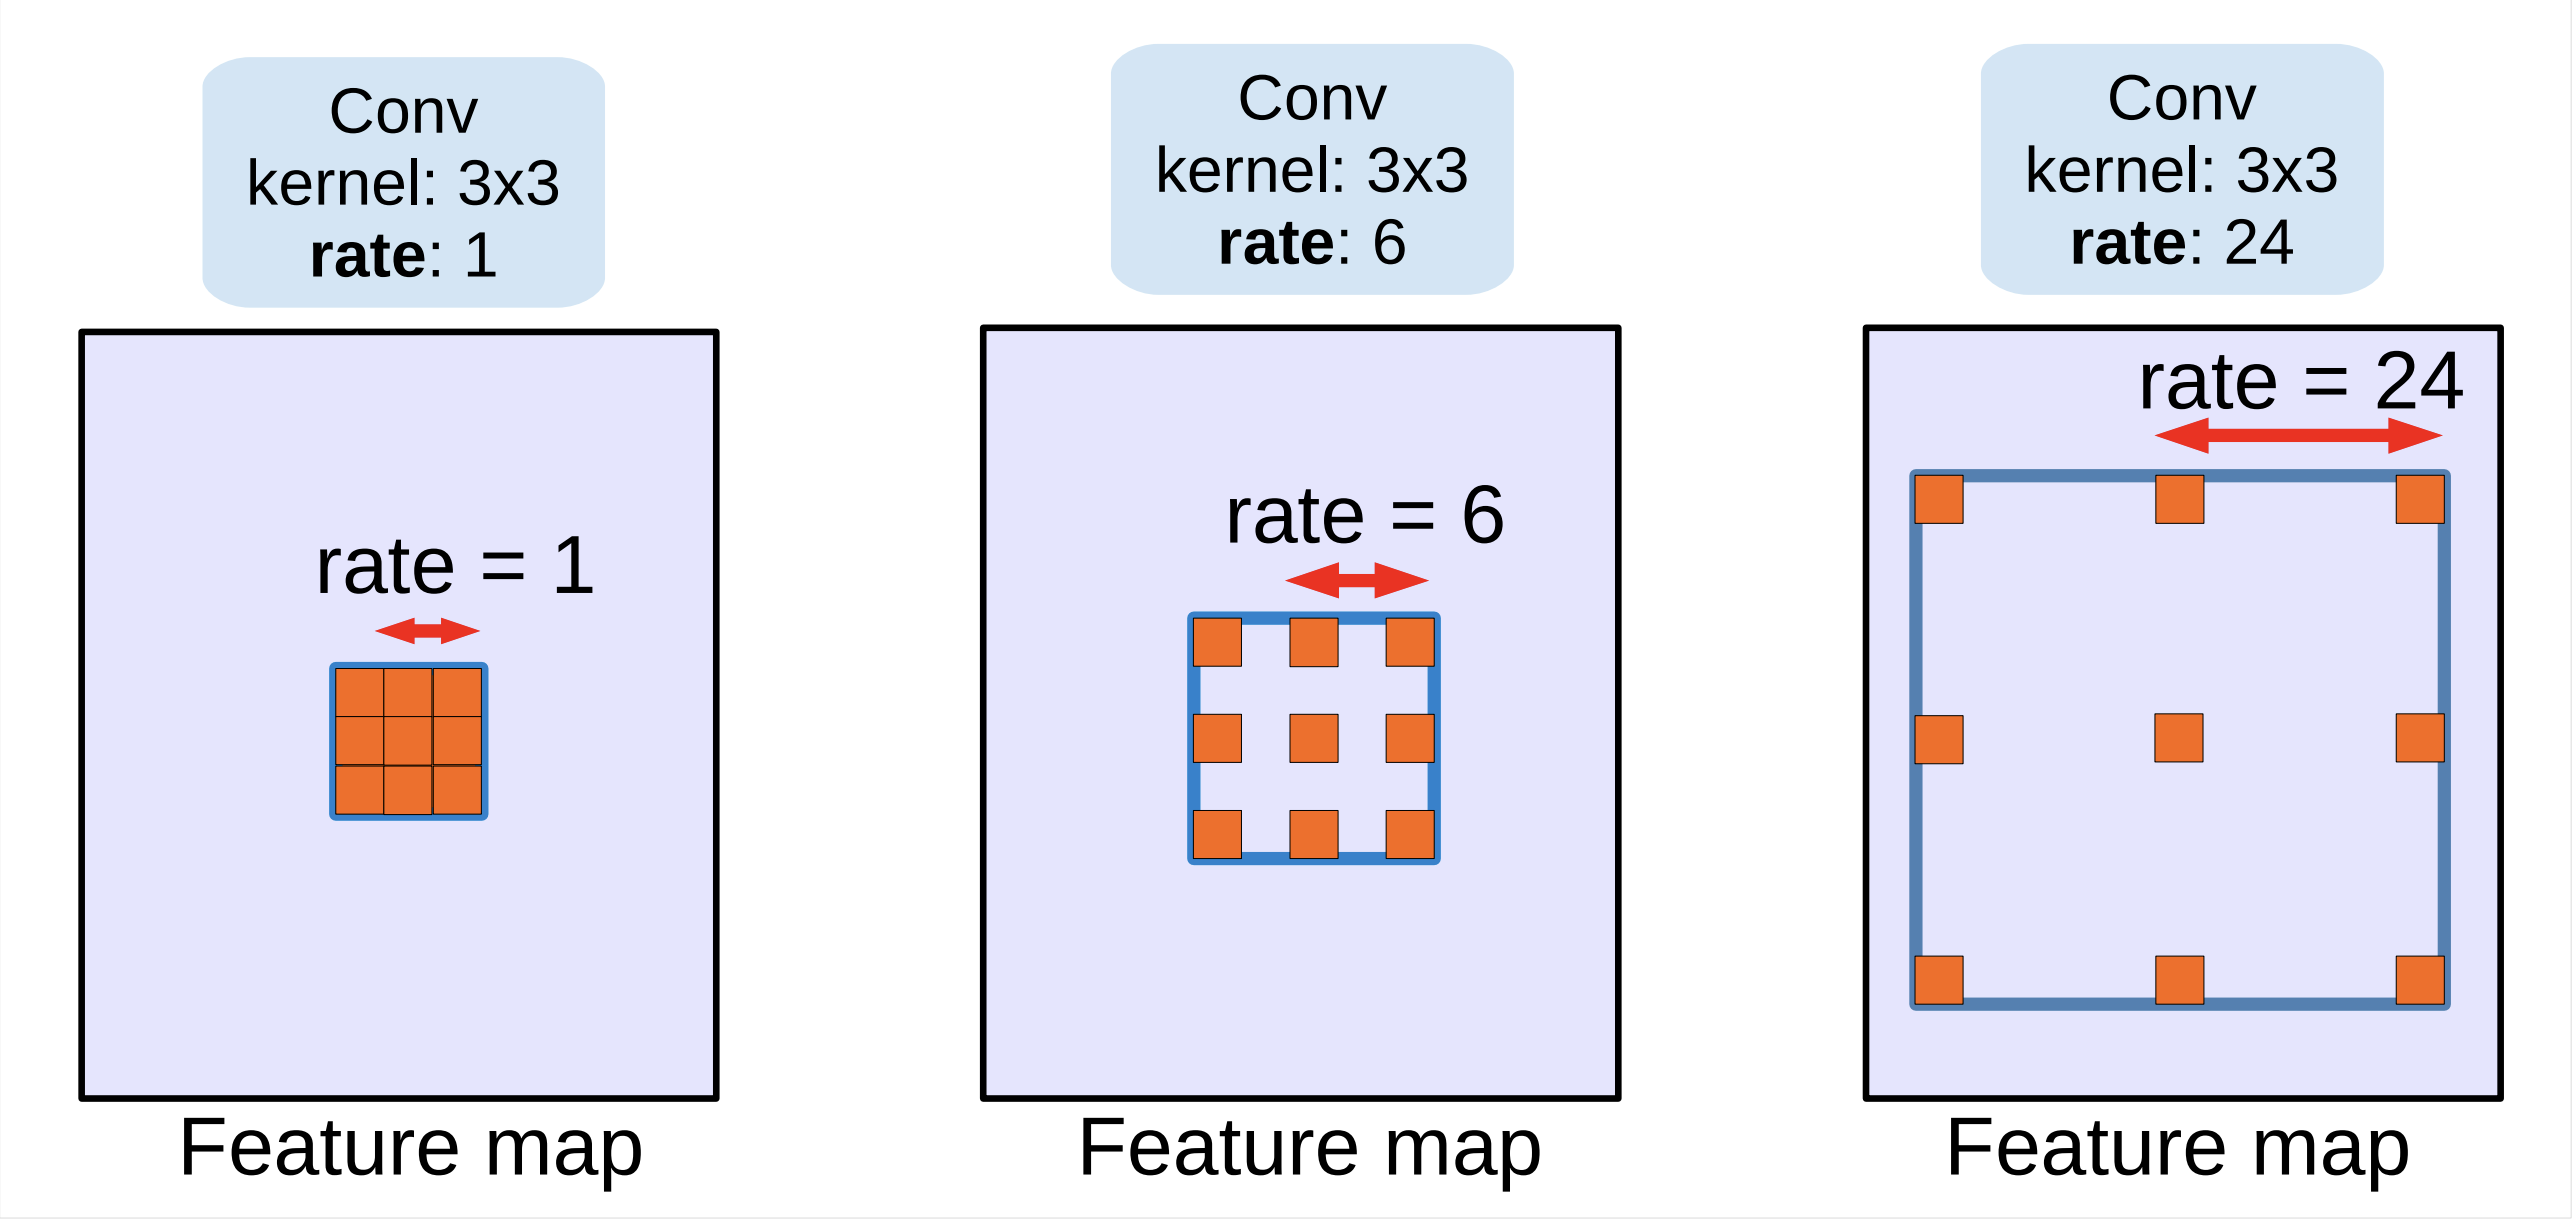
\includegraphics[width=0.85\textwidth]{atrous_convolution_chen.png}
  \caption{Atrous convolution with kernel size~3 at different dilation rates, from Chen et al. Standard convolution is an atrous convolution with rate~$=1$. Larger dilation rates allow the model to capture more global features through a wider field-of-view.}
  \label{fig:atrous_conv}
\end{figure}

DeepLabV3+ (Chen et al., 2018) combines the skip connections and encoder--decoder structure of U-Net with the \acrshort{aspp} module from its predecessor, fusing multi-scale context from \acrshort{aspp} with higher-resolution spatial detail from an earlier encoder layer to maintain both local and global spatial context. Both architectures use a ResNet backbone with ImageNet weights, reducing encoder training to a transfer learning task, while the decoder is trained from scratch to specialize in \acrshort{uvl} segmentation.

\begin{figure}[htbp]
  \centering
  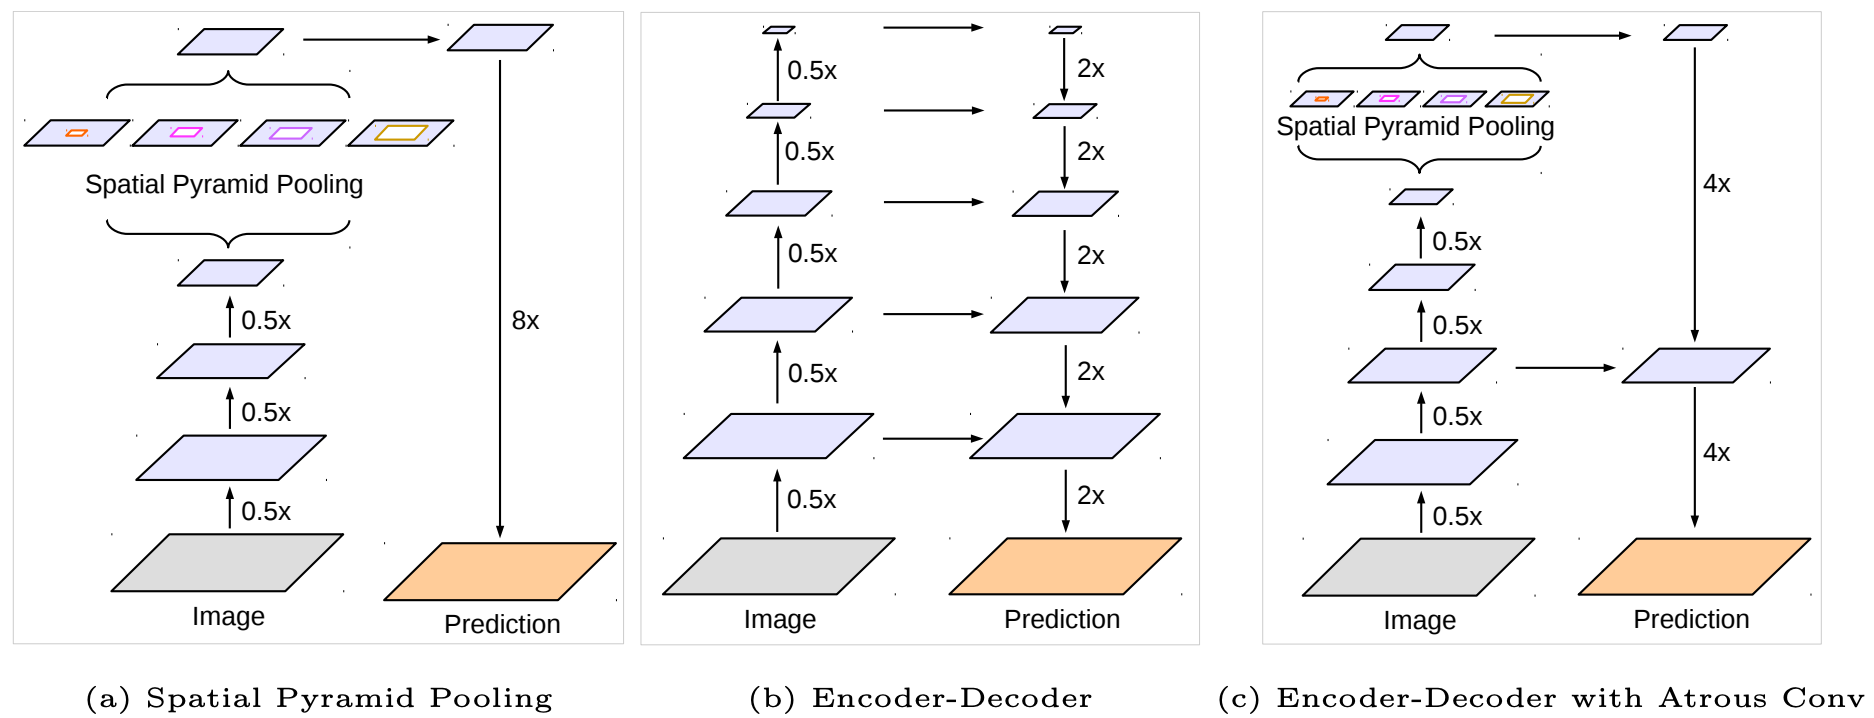
\includegraphics[width=\textwidth]{unet_deeplabv3.png}
  \caption{Comparison of U-Net and DeepLabV3+ architectures.}
  \label{fig:unet_deeplabv3}
\end{figure}

\section{Loss Functions}
\label{sec:loss}

Training uses a composite loss combining \acrshort{bce} with the Lov\'{a}sz-hinge loss:

\begin{equation}
  \mathcal{L} = w_{\text{bce}} \cdot \text{BCE}(y, p;\; \texttt{pos\_weight}) + w_{\text{lovasz}} \cdot \text{Lov\'{a}sz}(y, p)
  \label{eq:total_loss}
\end{equation}

\noindent where $y$ is the ground truth, $p$ is the predicted probability, and $w_{\text{bce}}$ and $w_{\text{lovasz}}$ are scalar weights (typically 0.5 each).

\paragraph{Binary Cross-Entropy.} The \acrshort{bce} term is modified with \texttt{pos\_weight\,=\,30}, which multiplies the loss contribution of positive (vacant) pixels by 30. Given the 3.4\% vacancy rate, this ensures that the relatively rare vacant pixels contribute meaningfully to the gradient signal. Without positive weighting, the optimizer would converge to predicting all pixels as non-vacant (the trivial solution).

\paragraph{Lov\'{a}sz-Hinge Loss.} The Lov\'{a}sz extension (Berman et al., 2018) provides a piecewise-linear convex surrogate to the Jaccard (\acrshort{iou}) loss. While cross-entropy optimizes per-pixel classification accuracy, the Jaccard index is a set-level metric that considers the ratio of intersection to union. Directly optimizing \acrshort{iou} is intractable, as it is discrete and non-differentiable, but the Lov\'{a}sz extension exploits the submodularity of the Jaccard set function to construct a tight convex surrogate---a continuous function that can be minimized by gradient descent.

The Lov\'{a}sz-hinge loss was preferred over the more common Dice loss for two reasons: (1)~it directly surrogates \acrshort{iou}, and (2)~empirically, it produced more stable threshold behavior during inference. Predictions trained with Lov\'{a}sz loss showed less sensitivity to threshold choice compared to Dice loss, which tended to produce probability distributions clustered near 0.5.

\section{Training Pipeline}
\label{sec:training}

All models were trained using the following pipeline:

\begin{itemize}
  \item \textbf{Optimizer:} AdamW with weight decay 0.01. Learning rate varied by experiment ($5 \times 10^{-4}$ to $10^{-3}$).
  \item \textbf{Learning rate schedule:} Cosine annealing (\texttt{CosineAnnealingLR}) with $T_{\max}$ set to the total number of planned epochs and $\eta_{\min} = 10^{-6}$.
  \item \textbf{Linear warmup (5 epochs):} The learning rate ramps linearly from 0.1\% to 100\% of the target learning rate over the first 5 epochs to prevent early training instability. High \texttt{pos\_weight} and class imbalance can produce large gradient spikes, especially with Lov\'{a}sz loss. The warmup period allows the model to establish a stable feature representation before encountering full-magnitude gradients.
  \item \textbf{Gradient clipping:} Per-step gradient norm clipping caps occasional extreme gradients, providing a hard safety bound on update magnitude.
  \item \textbf{Early stopping:} Training was monitored on the validation \acrshort{iou} with a patience of 40 epochs. The model checkpoint with the highest validation \acrshort{iou} was retained.
  \item \textbf{Data augmentation:} Random horizontal flips and 90-degree rotations were applied during training. Color jitter was deliberately excluded because spectral values in \acrshort{naip} imagery carry physical meaning (surface reflectance), and random color perturbation would corrupt this information.
  \item \textbf{Band dropout ($p = 0.3$):} During training, each input band was independently zeroed with probability~0.3, preventing the model from relying on any single band and encouraging learning of redundant spectral representations.
  \item \textbf{Hardware:} Models were trained on an NVIDIA Titan RTX (24~GB VRAM) and an NVIDIA Titan V (12~GB VRAM). At $512\times512$ patch size, batch sizes of 4--8 were used; at $1024\times1024$, batch sizes of 2--8 depending on backbone depth.
\end{itemize}

\subsection{Class Imbalance Strategy}
\label{sec:class_imbalance}

With only 3.4\% of training pixels labeled vacant, class imbalance is a central challenge. Multiple complementary strategies were employed:

\begin{enumerate}
  \item \textbf{Vacant patch augmentation:} During training, patches containing a reasonable number of vacant pixels were oversampled and augmented, increasing the proportion of vacant pixels seen per epoch.
  \item \textbf{Positive weight in \acrshort{bce} loss (\texttt{pos\_weight\,=\,30}):} Amplifies the gradient contribution of vacant pixels by 30$\times$, preventing the trivial all-non-vacant solution.
  \item \textbf{Ignore masking:} Roads, water, eroded boundaries, and known label errors are masked out, preventing the model from learning spurious associations with these surfaces.
  \item \textbf{Lov\'{a}sz-hinge loss:} Directly surrogates \acrshort{iou}, which is inherently sensitive to the minority class. A model that predicts no vacant pixels receives $\text{IoU} = 0$.
\end{enumerate}

\subsection{Inference}
\label{sec:inference}

At inference time, predictions are generated using overlapping tiles with a stride equal to half the patch size. A Gaussian-weighted averaging is applied to reduce boundary artifacts, assigning lower weight to patch edges where predictions are inherently weaker due to limited spatial context. The final probability map is then thresholded to produce binary predictions. The threshold is selected on the validation set by sweeping from 0.01 to 0.99 and choosing the value that maximizes the target metric ($F_1$ or $F_2$).

\chapter{Results}
\label{ch:results}

\section{Overview}
\label{sec:results_overview}

DeepLabV3+ at 1024~px patch size achieved the best results with consistent $F_2$ scores above 40\%. U-Net outperformed DeepLabV3+ in both the 256 and 512 patch sizes, exemplifying DeepLabV3+'s need for a larger global receptive field and U-Net's superior performance at local spatial scales.

\begin{table}[htbp]
  \centering
  \caption{Selected model runs and ablations. All DeepLabV3+ runs used ResNet-50; all U-Net runs used ResNet-34. $F_2$ is calculated at its optimal threshold; $F_1$ and Test IoU are evaluated at threshold~0.5. Best results in bold.}
  \label{tab:selected_runs}
  \begin{tabular}{llcccrrr}
    \toprule
    \textbf{Run} & \textbf{Arch} & \textbf{Patch} & \textbf{Mask} & \textbf{Ch} & \textbf{$F_2$} & \textbf{$F_1$} & \textbf{Test IoU} \\
    \midrule
    \textbf{d\_27} & \textbf{DLV3+} & \textbf{1024} & \textbf{v2} & \textbf{5} & \textbf{42.3} & \textbf{27.79} & \textbf{16.14} \\
    u\_29 & U-Net & 512 & v2 & 5 & 39.0 & 21.75 & 12.20 \\
    u\_32 & U-Net & 512 & v2 & 4 & 38.2 & 23.04 & 13.02 \\
    u\_15 & U-Net & 512 & v1 & 4 & 34.57 & 22.67 & 12.78 \\
    d\_15 & DLV3+ & 1024 & v1 & 4 & 35.65 & 23.87 & 13.55 \\
    d\_10 & DLV3+ & 512 & v1 & 4 & 30.17 & 19.18 & 10.61 \\
    \bottomrule
  \end{tabular}
\end{table}

\Cref{tab:selected_runs} presents six runs isolating the effect of patch size, mask version, and building probability channel. For DeepLabV3+, increasing patch size from 512 to 1024~px improved test $F_2$ from 30.2 to 35.7 (runs d\_10$\rightarrow$d\_15), a gain of 5.5 points, consistent with the \acrshort{aspp} module requiring larger spatial context to be effective. The v1 mask U-Net at 512~px (u\_15, $F_2$=34.6) performed comparably to DeepLabV3+ at 1024~px (d\_15, $F_2$=35.7), suggesting that at this stage the gains from larger patches and stronger architecture were roughly equivalent. Upgrading to the v2 mask and adding the building probability channel together lifted DeepLabV3+ from 35.7 to 42.3 (runs d\_15$\rightarrow$d\_27, +6.6 points); the building probability channel's isolated contribution is estimated at 0.8 points from the U-Net pair at 512~px with the v2 mask (u\_32 vs.\ u\_29, 38.2$\rightarrow$39.0). The best result overall, run d\_27, combines all improvements and achieves test $F_2$~42.3, $F_1$~27.8, and IoU~16.1 at threshold~0.298.

\section{Experimental Progression}
\label{sec:progression}

Over 30+ training runs (see \Cref{appendix:all_runs}), experiments progressed through three phases.

\paragraph{Phase 1} kept patch size constant at 256~px (153~m, 23,500~m\textsuperscript{2} at 0.6~m/px) while tuning backbone depth, input channels, loss composition, and oversampling rate. \acrshort{bce} + Lov\'{a}sz loss consistently outperformed \acrshort{bce} + Dice and pure Dice. A \texttt{pos\_weight} of 30 was found to be optimal. Four-band input (RGBN) matched or outperformed 10-band input with spectral features, indicating that additional bands introduced more noise than signal. U-Net with a ResNet-34 backbone outperformed DeepLabV3+ variants, consistent with DeepLabV3+'s \acrshort{aspp} module being better suited for larger spatial contexts.

\paragraph{Phase 2} increased patch size from 256 to 512 (307~m) and 1024 (614~m). For DeepLabV3+/ResNet-50, test $F_2$ improved from 0.302 at 512~px (run d\_10) to 0.357 at 1024~px (run d\_15), a substantial growth as the \acrshort{aspp} module benefited from the larger spatial extent. U-Net performance peaked at 512~px. Visual inspections of u\_15 predictions revealed systematic false positives attributable to labeling errors in the vacancy mask, motivating the refinements for mask v2.

\paragraph{Phase 3} corrected 67 parcels in the v2 vacancy mask and introduced planimetric roadbed masking. Concurrent with mask refinement, runs d\_19 and d\_20 collapsed at epoch~2 under an identical configuration to run d\_18, which had converged normally over 117 epochs. This demonstrated sensitivity to random initialization under \texttt{pos\_weight=30} with Lov\'{a}sz loss. Linear LR warmup and gradient clipping resolved this instability; no subsequent run collapsed. A 5th input channel encoding building presence probability was introduced for ablation against 4-channel baselines. For U-Net/ResNet-34 at 512~px with the v2 mask, the 5-channel model (run u\_29, $F_2$~0.390) outperformed its 4-channel counterpart (run u\_32, $F_2$~0.382) by 0.008, a small but consistent gain.

The best overall result was DeepLabV3+/ResNet-50 run~027 (1024~px, 5-channel, v2 mask, LR warmup, gradient clipping): test $F_2$~0.423, an improvement of 0.066 over the best Phase~2 checkpoint.

\acrshort{ap} values are low across all runs (best \acrshort{ap}~0.217, run d\_24), but this does not straightforwardly indicate poor discriminative ability. \acrshort{ap} is bounded below its theoretical maximum by irreducible label noise: the model's high-confidence vacant predictions include parcels that appear visually vacant but are administratively non-vacant. These are counted as false positives at all thresholds, deflating precision throughout the PR curve and suppressing \acrshort{ap} regardless of model quality. \acrshort{ap} is best interpreted here as a relative measure between models and as a lower bound on true discriminative ability.

Precision remains low (highest 36\%) across all runs. This is the fundamental constraint of the task: many non-vacant surfaces are spectrally identical to vacant land, establishing a floor on the false positive rate. At these precision levels, roughly 4--6 out of every 7 pixels predicted vacant are false positives at the pixel level.

\section{Qualitative Analysis}
\label{sec:qualitative}

The $F_2$-thresholded predictions of the best model run, DeepLabV3+ d\_27, are shown in \Cref{fig:deeplab_error}. The model produces spatially coherent predictions and demonstrates several expected behaviors. It does not predict vacancy where buildings are present, and correctly classifies large urban features that could plausibly be confused with vacant land: Prospect Park, Sunset Park, and Green-Wood Cemetery are all predicted as non-vacant, as are soccer, baseball, and football fields. Inconsistencies appear at smaller recreational features---basketball and tennis courts are predicted as vacant in some locations and non-vacant in others, with no clear spatial pattern.

The primary source of false positives is industrial land, concentrated along the Brooklyn waterfront and, in the Bronx, around Hunts Point. Parking lots constitute a second category of false positives, with prediction confidence appearing to correlate inversely with lot structure: large lots with visible lane markings and ordered vehicle placement tend to be classified as non-vacant, while smaller or less-organized lots are consistently predicted as vacant. Small patches of dense tree cover are occasionally predicted as vacant, though large contiguous canopy is correctly rejected.

Among false negatives, the model most consistently misses grassy vacant lots. Dirt lots and mixed dirt-grass lots with higher bare soil coverage are detected more reliably than lots with predominantly grass cover. Narrow vacant lots are also frequently missed, appearing as isolated false negatives scattered across the prediction map.

\begin{figure}[htbp]
  \centering
  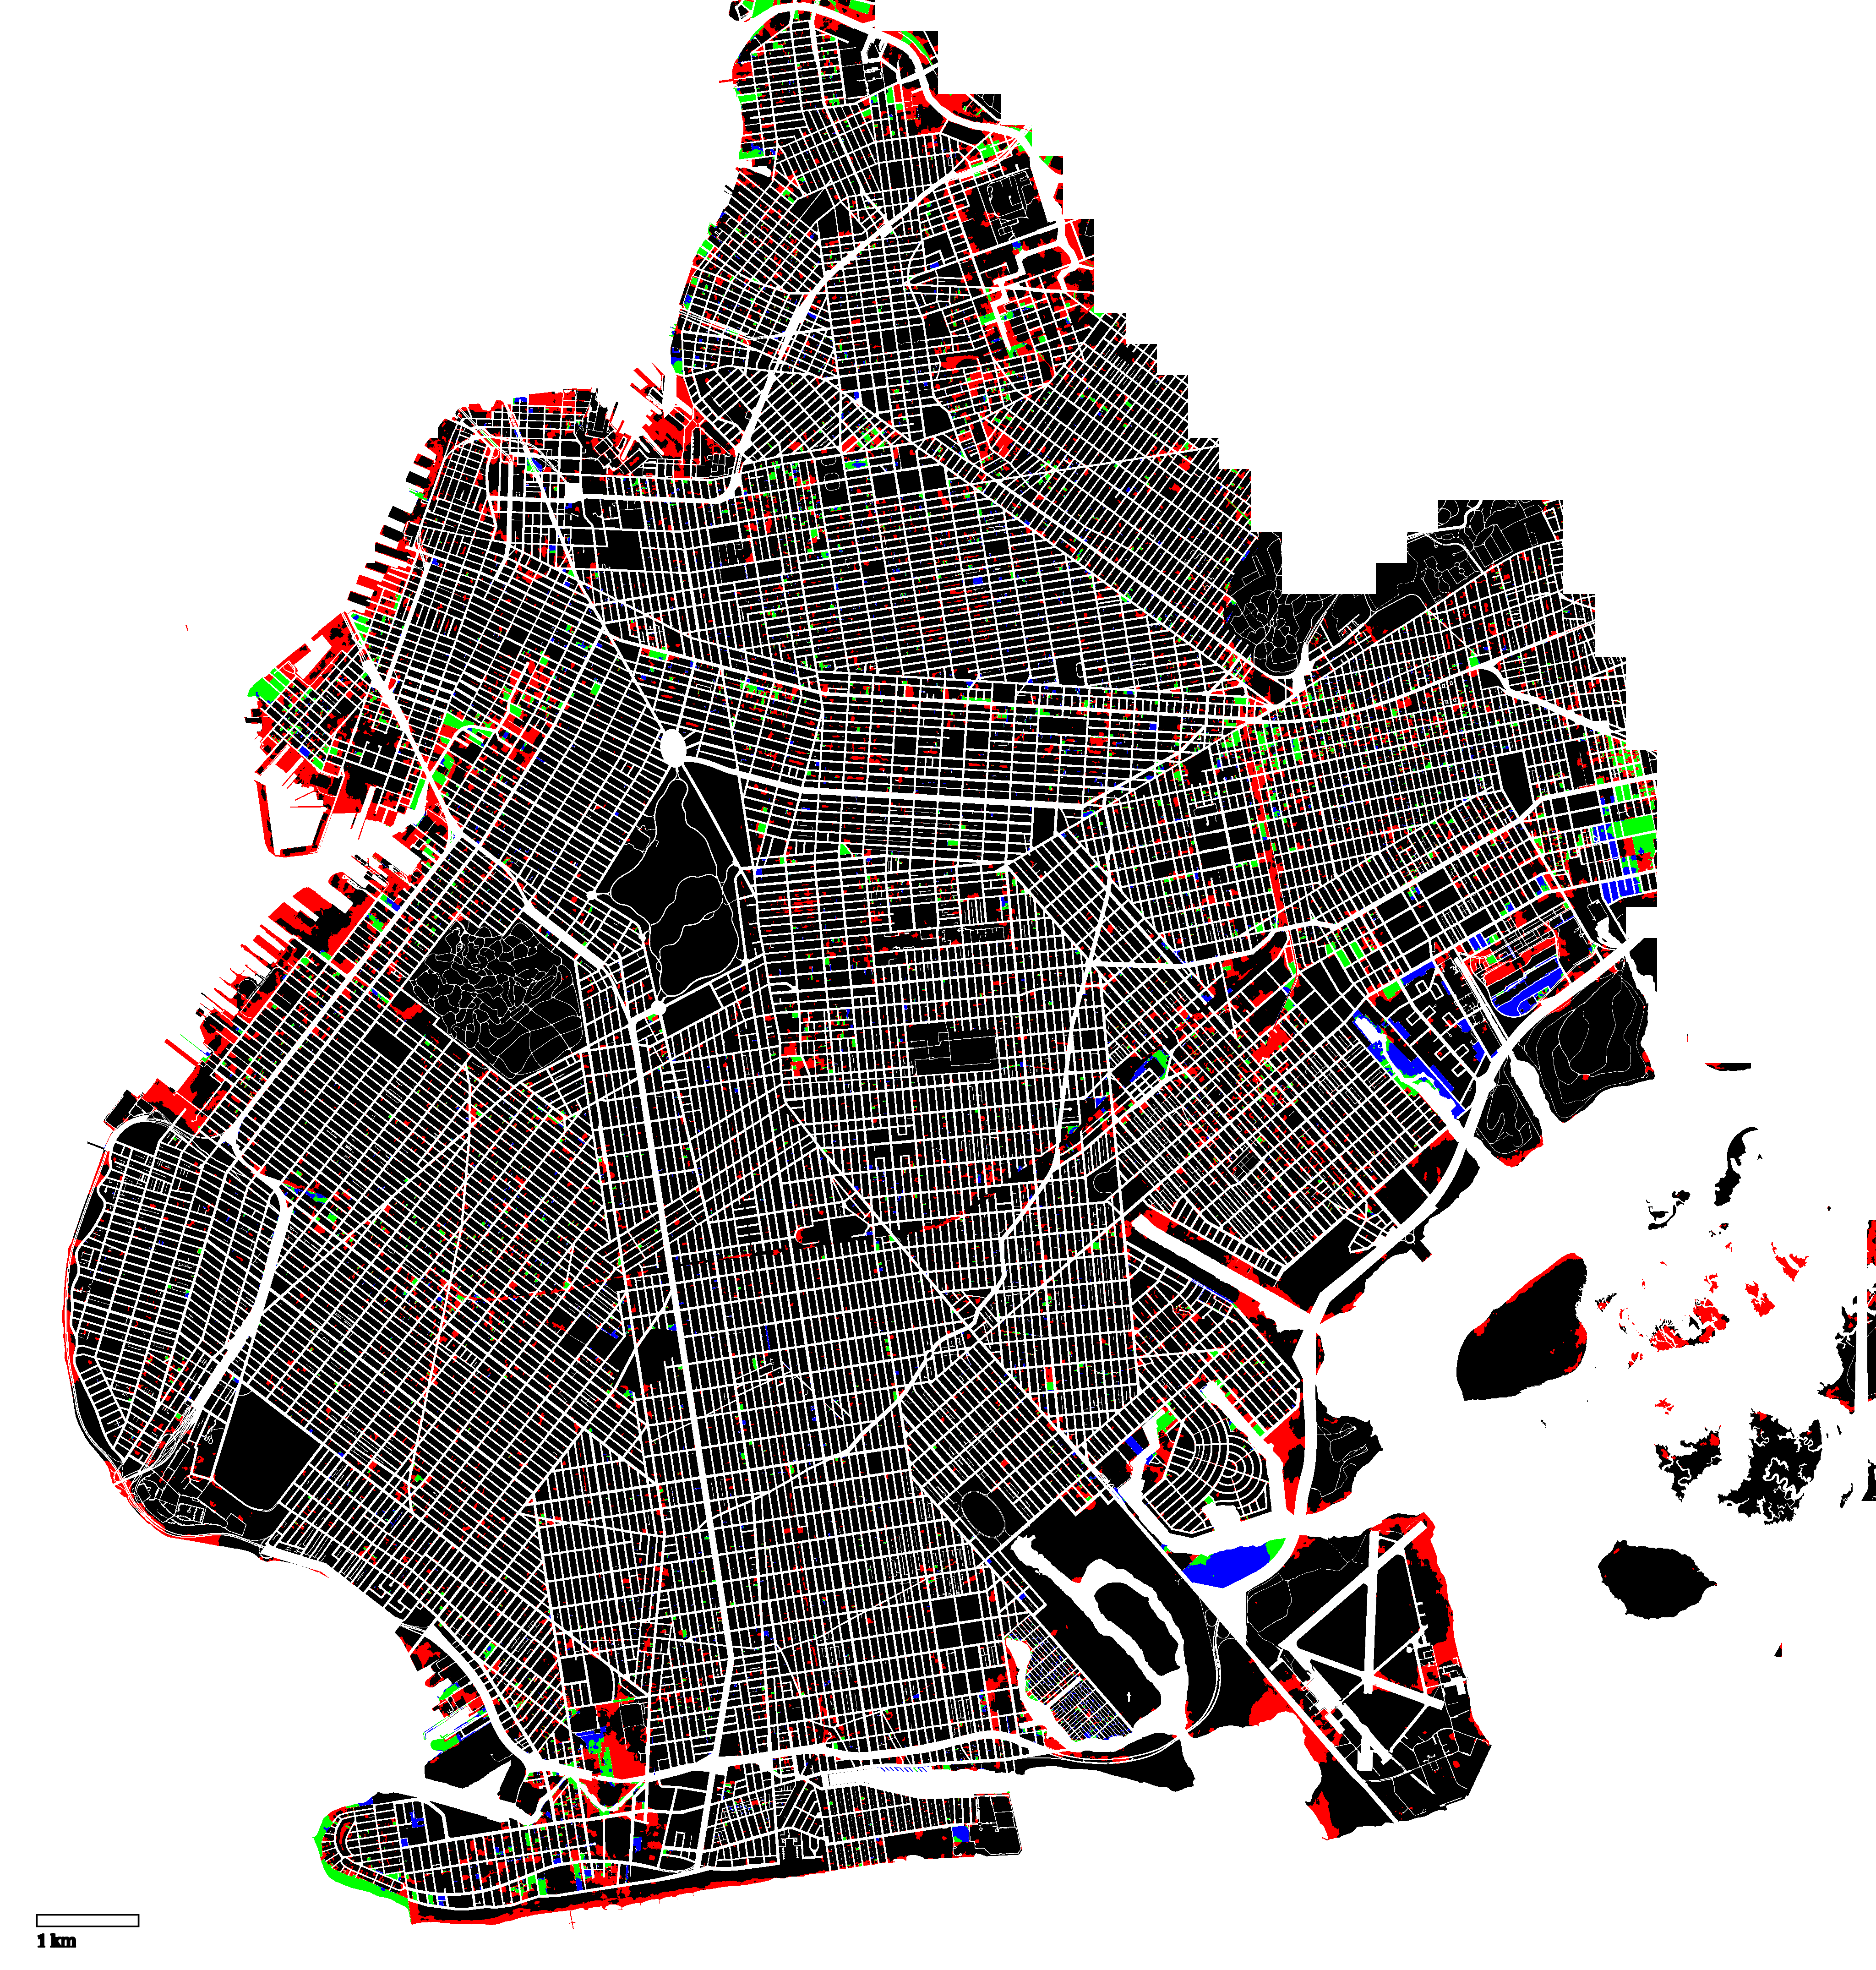
\includegraphics[width=\textwidth]{deeplab_27_error_s512_t298.png}
  \caption{Error map for DeepLabV3+ run d\_27, evaluated on Brooklyn at threshold~0.298. Black represents pixels correctly predicted as non-vacant (TN). Green indicates correct vacant predictions (TP). Blue denotes missed vacant pixels (FN), and red represents false positives (FP).}
  \label{fig:deeplab_error}
\end{figure}

\chapter{Discussion}
\label{ch:discussion}

\section{Interpreting the Failure Modes}
\label{sec:failure_modes}

The model has several failure modes for different reasons. The parking lot false positive pattern is not straightforwardly a model failure. Unlined, disorganized lots---unpaved or with haphazardly parked vehicles---share the spectral and textural signature of vacant land, and in many cases the administrative distinction is equally ambiguous: MapPLUTO classifies some outdoor parking lots under the G7 vacancy code while visually identical adjacent lots with active commercial use are classified as non-vacant. The model's confusion therefore partly reflects genuine definitional overlap between unattended outdoor parking and vacant land with asphalt cover, not a learnable distinction from aerial imagery alone.

Large industrial facilities generate false positives due to their bare concrete expanses, scattered equipment, and irregular vehicle staging areas. For a planning application this failure mode is relatively benign: a New York City planner reviewing model output would recognize an industrial waterfront immediately.

Soccer, football, and baseball diamonds are correctly classified, but standalone basketball and tennis courts are frequently mislabeled. Targeted augmentation of sports facility examples, potentially with OSM data, could reduce this failure mode.

The model's inconsistent detection of grassy vacant lots is the most operationally significant false negative pattern. Dirt lots are reliably detected; mixed grass-and-dirt lots are inconsistent; purely grassy lots are frequently missed entirely. The model has apparently learned bare soil as a strong vacancy signal but has not learned a robust representation of vegetated vacancy. This may reflect the training label distribution from Queens, spectral ambiguity between grassy vacancy and maintained green space, or both. The SWIR band, which discriminates between soil moisture states and surface cover types that overlap in the visible and \acrshort{nir}, could partially address this, but no freely available high-resolution national imagery currently provides it.

Small and narrow lots present a hard resolution constraint. At 0.6~m/pixel, a lot 4~meters wide occupies approximately 7~pixels across its short dimension---insufficient for the model to build a spatial representation distinguishable from adjacent developed land, particularly given relief distortion from surrounding structures. Higher-resolution \acrshort{naip} imagery (0.3~m) would double the effective pixel count for narrow lots and could ameliorate this limitation.

\section{Label Noise as a Performance Ceiling}
\label{sec:label_noise_ceiling}

Several categories of prediction error reflect noise in the ground truth rather than model deficiency. Parcels under active construction at the time of imagery are labeled vacant in MapPLUTO but visually resemble neither vacant land nor completed structures. Parcels labeled vacant that clearly contain buildings represent assessor lag. Community-used lots, informally maintained by residents as painted courts or murals, are labeled vacant administratively but rejected by the model based on visual evidence of active use. In each case, the model's prediction is arguably more accurate than the label.

This represents a fundamental tension in the task formulation: administrative vacancy (derived from tax records and assessor visits) and visual vacancy (derivable from aerial imagery) are related but not equivalent concepts. The model is trained and evaluated on one, but in reality the latter could be more helpful for \acrshort{uvl} repurposing.

\section{Practical Deployment}
\label{sec:deployment}

At the $F_2$-optimal threshold (0.298 for run~027), the model maximizes recall at the cost of precision, surfacing the largest possible fraction of vacant parcels for human review. At the $F_1$-optimal threshold, precision and recall are more balanced and the false positive burden on a reviewer is lower, but more vacant parcels are missed. The choice between operating points is a workflow decision that depends on the scale and purpose of the application.

For city-wide screening across an entire borough, the high false positive rate at the $F_2$-optimal threshold may produce a shortlist too large for practical review. In this context, the $F_1$-optimal threshold---or a higher threshold still---reduces reviewer burden at the cost of missing some fraction of vacant parcels. Conversely, for targeted applications such as rezoning a specific industrial corridor, identifying candidate parcels for bioswale installation along a flood-prone highway, or auditing a single neighborhood for infill development potential, the $F_2$-optimal threshold is appropriate: the geographic scope is bounded, the reviewer is already familiar with the area, and missing a vacant parcel is more costly than reviewing a false positive.

In either case, model output is most useful when layered with existing GIS data. Overlaying predictions with zoning maps, building permits, and land use classifications would immediately resolve many false positives. Conversely, a grassy lot flagged in a high-demand residential neighborhood warrants closer inspection regardless of confidence score. The model's value lies in reducing the search space, not replacing the planner. Thus, the appropriate operating point should be chosen to match the capacity and scope of the review workflow it supports.

\section{Broader Implications}
\label{sec:implications}

The concentration of vacant lots identified by the model is geographically coherent with known patterns of urban disinvestment. The Broadway Junction area of Brooklyn and parts of the South Bronx, historically underserved and now experiencing early-stage gentrification pressure, show elevated vacancy density in the model output consistent with prior studies. This spatial coherence supports the model's validity even where pixel-level metrics are modest.

The policy relevance of vacant land identification extends beyond infill housing. Bioswale installation along flood-prone corridors, such as the 65th Place corridor near the BQE---a chronic pluvial flooding site in New York---would require identification of adjacent \acrshort{uvl}. Stormwater infrastructure sited on vacant land has lower acquisition cost and lower displacement risk than development on occupied parcels. The model's false positives for parking lots and industrial land are less consequential for stormwater screening than for housing: a parking lot adjacent to a highway is a plausible bioswale site regardless of its vacancy status.

While the model presented here can identify vacant land, identification is only the first step. Vacant land in New York City is predominantly privately owned, and conversion to housing, green infrastructure, or community use requires acquisition, negotiation, or policy intervention. The socioeconomic dimensions of redevelopment---displacement risk, neighborhood income effects, equitable distribution of amenities---are not captured by the model. A screening tool that surfaces vacant land without accounting for these factors risks reinforcing rather than remedying spatial inequity.

\section{Future Work}
\label{sec:future_work}

The most impactful near-term improvement is further label refinement. The v2 mask corrections improved performance substantially, and the parcel-level error analysis has identified additional candidates for ignore masking or label conversion. A structured annotation pipeline targeting the highest-confidence false positives and false negatives could ease this process and speed up mask refinement.

While the focus here is open source, SWIR data could be acquired through private vendors to add imperviousness signals. Testing alternative encoders such as Xception, recommended by the authors of DeepLabV3+, could also improve performance. Finally, extending evaluation to a second city would test generalizability of the learned features beyond New York's specific urban fabric.

\chapter{Conclusion}
\label{ch:conclusion}

This study presents the first application of deep learning segmentation to vacant lot detection in dense American urban fabric. While prior work has focused largely on cities with coarser urban form, the fine-grained, mixed-use parcel structure of cities like New York poses a unique challenge. Using freely available \acrshort{naip} aerial imagery and administrative vacancy records from MapPLUTO, a DeepLabV3+/ResNet-50 model trained on Queens and evaluated on Brooklyn achieves a test $F_2$ of 42.3\%, while demonstrating spatially coherent predictions.

The results reveal that administrative vacancy is partially but not fully recoverable from aerial imagery: bare-soil and structurally distinct vacant lots are reliably detected, while grassy lots, narrow parcels, and cases where administrative and visual vacancy diverge represent a performance ceiling that is as much a labeling problem as a modeling one.

Deployed as a screening tool rather than an autonomous classifier, and calibrated to the scale and purpose of the planning application, the model could meaningfully reduce the search space for vacancy identification in cities that lack systematic ground-level survey capacity. The open-source release of the training pipeline, vacancy masks, and model weights is intended to lower the barrier for other northeastern cities looking into urban infill development.


% =============================================================
% APPENDICES
% =============================================================
\appendix

\chapter{Manual Mask Corrections}
\label{appendix:manual_corrections}

\begin{figure}[htbp]
  \centering
  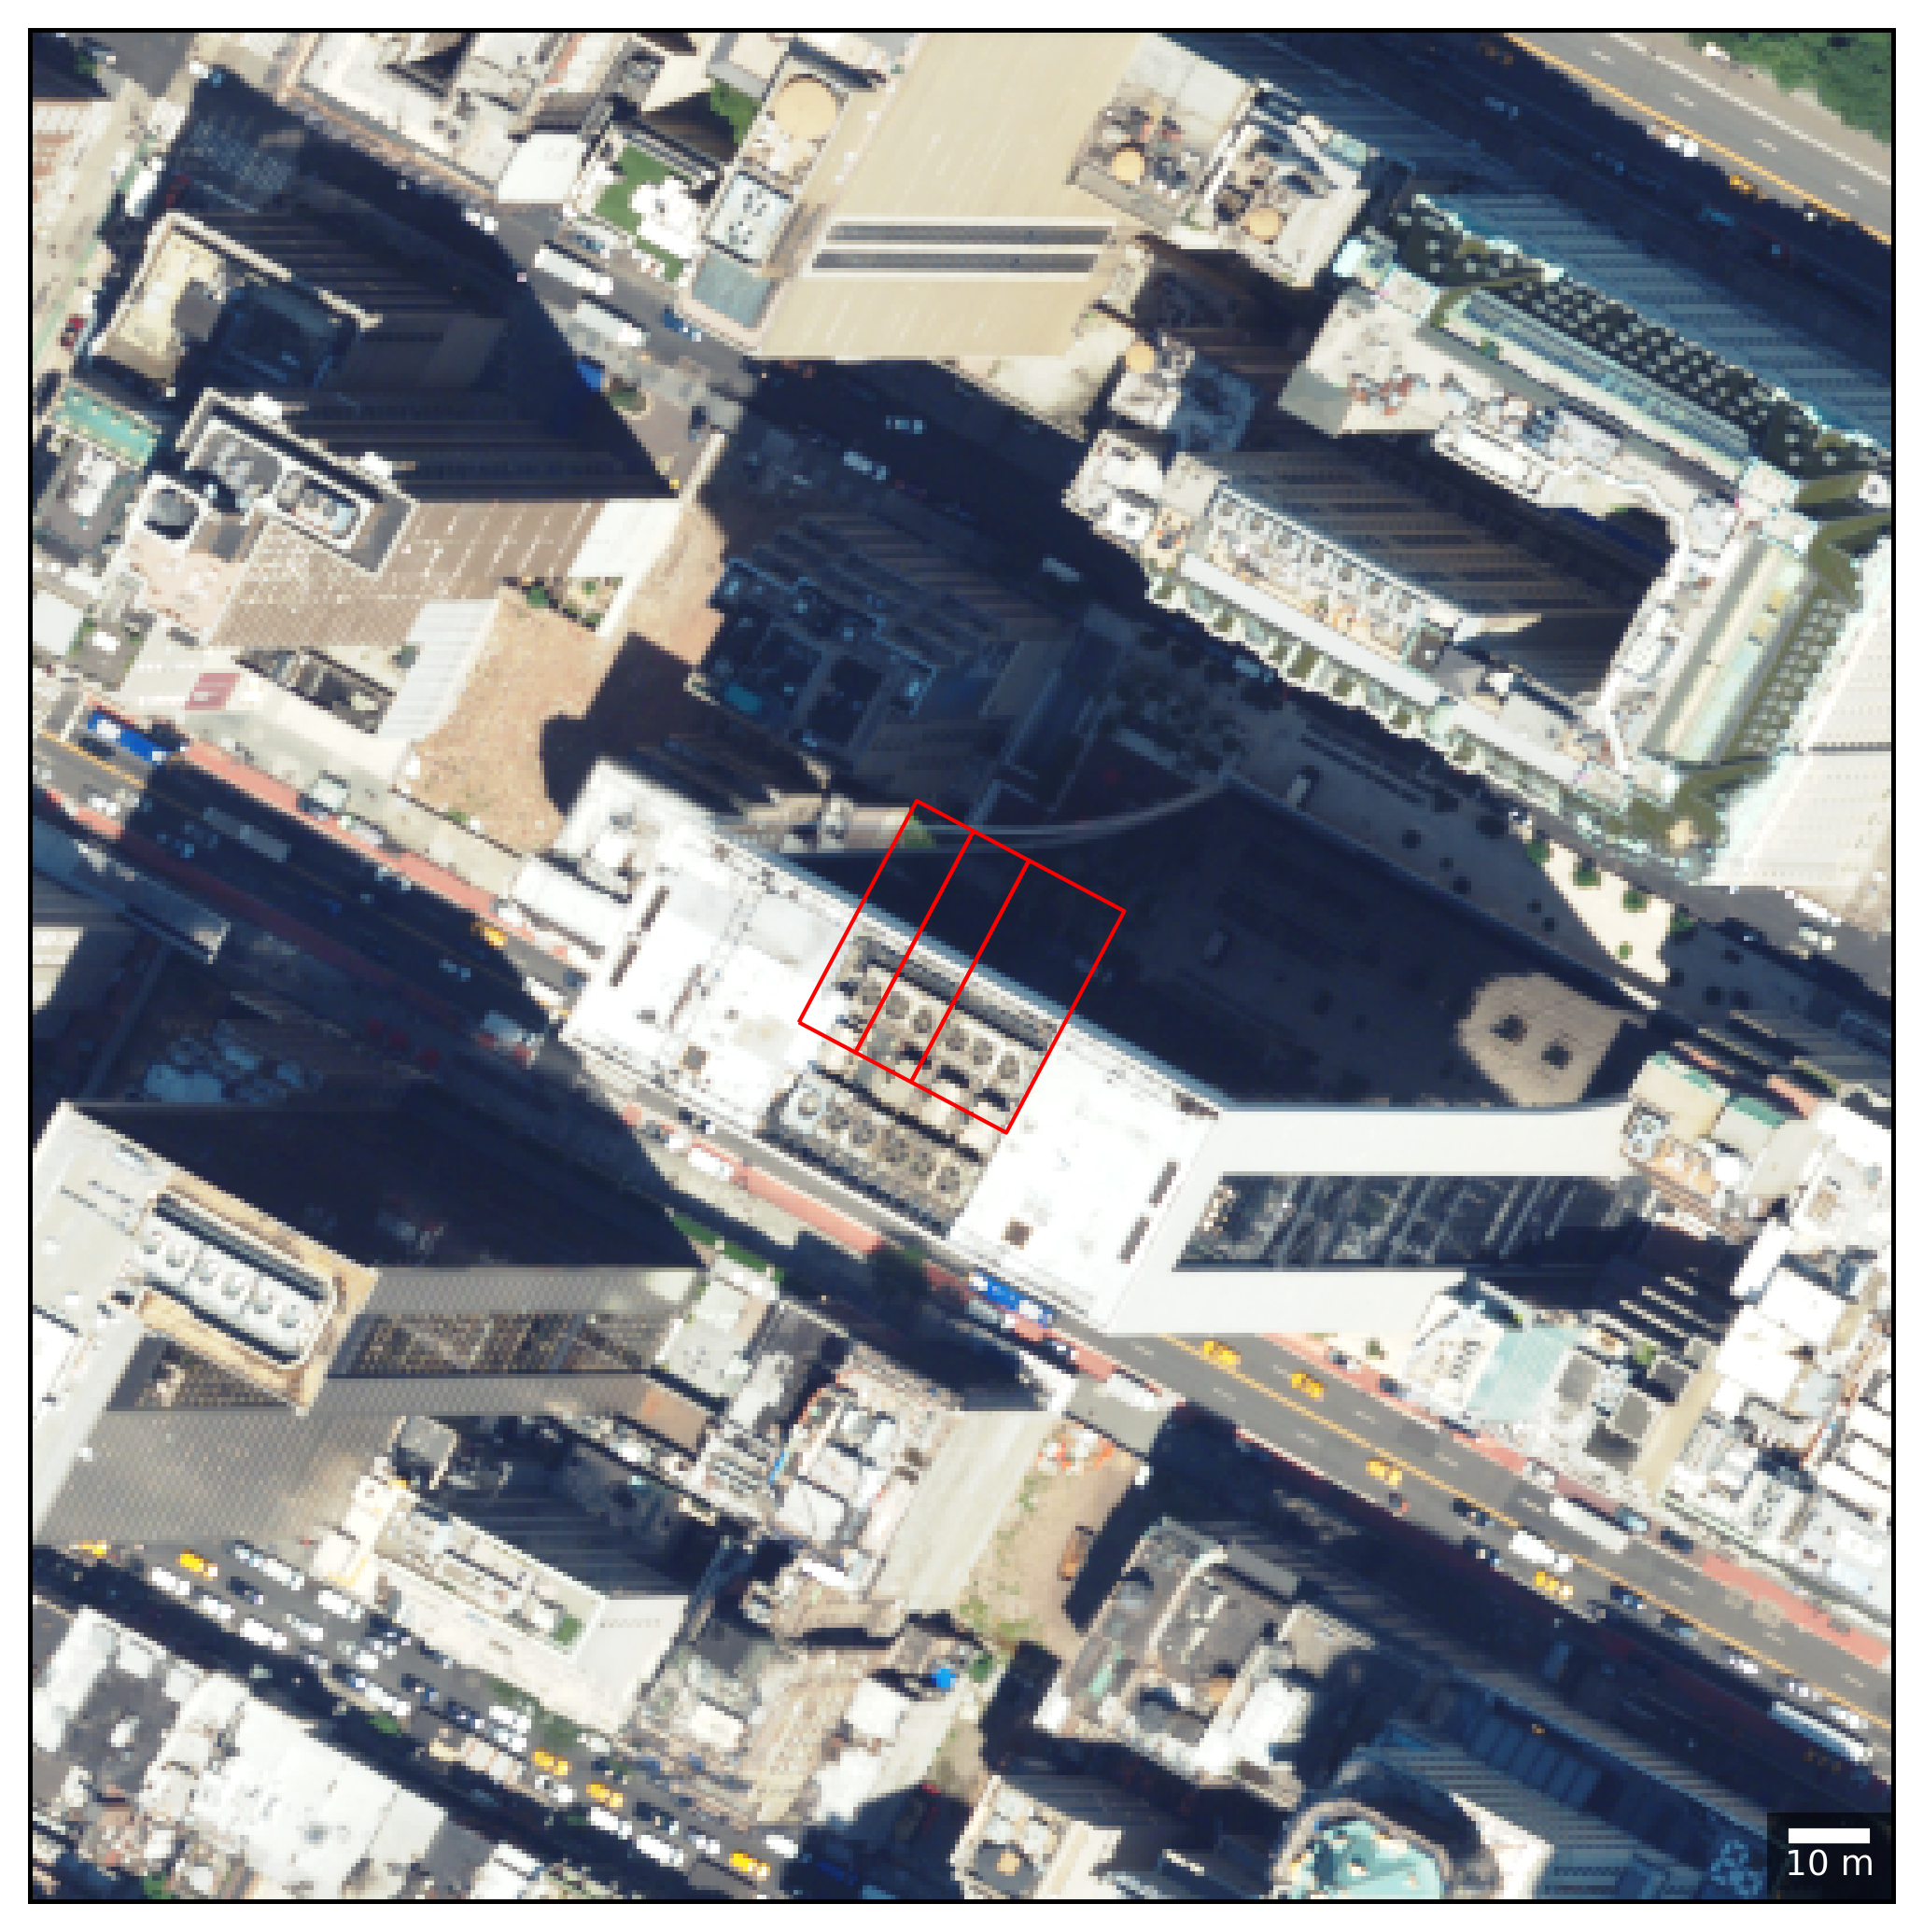
\includegraphics[width=0.85\textwidth]{omitted_shadow_lots.png}
  \caption{Example of vacant lots in shadow excluded from the mask and set to 255 (ignore). In areas with very tall buildings or sharp changes in elevation, relief displacement causes nearby lots to be partially or fully occluded in \acrshort{naip} imagery.}
  \label{fig:shadow_lots}
\end{figure}

Manual label corrections were applied as follows:
\begin{itemize}
  \item 11 parcels with clearly visible buildings were forced to non-vacant (0).
  \item 7 parcels confirmed as vacant through visual inspection or MapPLUTO version comparison (22v3 vs.\ 23v2) were forced to vacant (1).
  \item 49 parcels were set to ignore (255), including shadow-occluded parcels in Manhattan, parcels under active construction, parcels extending into water, and parcels obstructed by elevated highways.
\end{itemize}

\chapter{Parcel-Level Spectral Signal Validation}
\label{appendix:spectral_signal}

\section{Motivation}

Before investing in pixel-level segmentation, a preliminary analysis was conducted to determine whether \acrshort{naip} spectral features contain a supervised signal for distinguishing vacant from non-vacant parcels. The reasoning is conservative: if aggregated spectral statistics cannot separate vacancy at the parcel level, raw pixel values are unlikely to succeed either.

\section{Data Preparation}

The full MapPLUTO geodatabase (856,998 NYC tax lots) was joined with pre-computed spectral statistics from Google Earth Engine. The spectral statistics were computed by reducing \acrshort{naip} imagery over each parcel polygon, yielding per-parcel mean, median, and standard deviation for eight spectral bands and indices: R, G, B, \acrshort{nir}, \acrshort{ndvi}, \acrshort{savi}, Brightness, and BareSoilProxy.

The join on BBL (Borough-Block-Lot identifier) yielded 25,000 parcels with both spectral features and land-use labels. This sample was stratified during EDA to oversample vacant lots, ensuring the rare class had sufficient representation.

\section{Label Construction}

Binary labels were derived from the \texttt{BldgClass} column using the same vacant codes as the segmentation task (V0--V9, G7):
\begin{itemize}
  \item $1 =$ vacant (\texttt{BldgClass} matches a vacant code)
  \item $0 =$ not vacant
\end{itemize}
Of the 25,000 parcels, 500 (2.0\%) were labeled vacant.

\section{Feature Selection}

Sixteen features were selected---the mean and standard deviation of eight spectral bands/indices per parcel:
\begin{itemize}
  \item \textbf{Raw bands:} R, G, B, \acrshort{nir}
  \item \textbf{Derived indices:} \acrshort{ndvi}, \acrshort{savi}, Brightness, BareSoilProxy
\end{itemize}

Pixel count columns were excluded because count is a proxy for parcel area (geometric information). Since the segmentation model must generalize to cities without parcel data at inference time, geometric features were not permitted. Median columns were excluded as mean and standard deviation capture central tendency and heterogeneity sufficiently.

\section{Experimental Setup}

The dataset was split 80/20 with stratified sampling (\texttt{random\_state=42}), preserving the 2\% vacant fraction:
\begin{itemize}
  \item \textbf{Train:} 20,000 parcels (400 vacant, 2.0\%)
  \item \textbf{Test:} 5,000 parcels (100 vacant, 2.0\%)
\end{itemize}

Features were standardized using a \texttt{StandardScaler} fitted on the training set only. Three models were evaluated with \texttt{class\_weight="balanced"}:
\begin{itemize}
  \item Logistic Regression
  \item SVM with RBF kernel
  \item Random Forest (200 trees)
\end{itemize}

\section{Cross-Validation Results}

\begin{table}[htbp]
  \centering
  \caption{Cross-validation results (mean $\pm$ std across 5 folds).}
  \label{tab:cv_results}
  \begin{tabular}{lcc}
    \toprule
    \textbf{Model} & \textbf{$F_1$} & \textbf{AP} \\
    \midrule
    Logistic Regression & $0.149 \pm 0.005$ & $0.311 \pm 0.056$ \\
    SVM (RBF) & $0.212 \pm 0.013$ & $0.254 \pm 0.050$ \\
    Random Forest & $0.250 \pm 0.051$ & $0.306 \pm 0.028$ \\
    \bottomrule
  \end{tabular}
\end{table}

With a random baseline \acrshort{ap} of approximately 0.02 (equal to the positive class fraction), all models achieve \acrshort{ap} 10--15$\times$ above random, confirming that the spectral signal exists.

\section{Test Set Results}

\begin{table}[htbp]
  \centering
  \caption{Test set performance.}
  \label{tab:test_results}
  \begin{tabular}{lcccc}
    \toprule
    \textbf{Model} & \textbf{$F_1$} & \textbf{AP} & \textbf{Precision} & \textbf{Recall} \\
    \midrule
    Logistic Regression & 0.159 & 0.320 & 0.09 & 0.74 \\
    SVM (RBF)           & 0.215 & 0.212 & 0.13 & 0.69 \\
    Random Forest       & 0.290 & 0.346 & 0.61 & 0.19 \\
    \bottomrule
  \end{tabular}
\end{table}

\textbf{Logistic Regression} (precision=0.09, recall=0.74) casts a wide net---it catches 74\% of vacant parcels but 91\% of its ``vacant'' predictions are false positives. \textbf{SVM} (precision=0.13, recall=0.69) shows marginally better precision at slightly lower recall. \textbf{Random Forest} (precision=0.61, recall=0.19) adopts the opposite strategy---very conservative predictions but correct 61\% of the time when it does predict ``vacant.''

\section{Feature Importance}

The Gini importance scores from the trained Random Forest reveal that \textbf{standard deviation features dominate} the importance rankings. \texttt{Brightness\_stdDev} is the single most important feature, and the stdDev features collectively outweigh the mean features.

Standard deviation captures within-parcel spectral heterogeneity---a proxy for spatial texture. Vacant lots tend to have high spectral variance (mix of bare soil patches, weeds, debris, scattered materials), while non-vacant parcels with buildings tend to have more uniform spectral signatures. This finding directly motivates the pixel-level segmentation approach adopted in this thesis: the most important parcel-level features are \emph{proxies} for spatial texture. A convolutional segmentation model operating on raw pixel patches accesses the actual spatial texture directly.

\section{Summary}

\begin{table}[htbp]
  \centering
  \caption{Summary of parcel-level spectral signal validation.}
  \label{tab:spectral_summary}
  \begin{tabular}{p{4cm}p{9cm}}
    \toprule
    \textbf{Finding} & \textbf{Detail} \\
    \midrule
    Spectral signal exists & AP 10--15$\times$ above random baseline \\
    Best parcel-level model & Random Forest ($F_1$=0.29, AP=0.35, precision=0.61) \\
    Most important features & StdDev features (spectral heterogeneity), especially \texttt{Brightness\_stdDev} \\
    Key limitation & Low recall (19\%)---many vacant parcels are spectrally ambiguous when averaged \\
    Implication for segmentation & StdDev dominance indicates spatial texture is the critical discriminator \\
    \bottomrule
  \end{tabular}
\end{table}

\chapter{Pixel-Level Baseline Models}
\label{appendix:tree_baselines}

\section{Motivation}

Before training convolutional neural networks, two tree-based ensemble models were evaluated as pixel-level baselines. These models classify each pixel independently based on its spectral feature vector, without any spatial context from neighboring pixels. The purpose is to quantify how much of the vacancy signal is accessible from per-pixel spectral values alone and to establish a lower bound against which the CNN architectures are compared.

\section{Feature Set}

Each pixel was represented by a 10-dimensional feature vector: 4 \acrshort{naip} bands (R, G, B, \acrshort{nir}, normalized to $[0,\,1]$) and 6 spectral indices (\acrshort{ndvi}, \acrshort{savi}, Brightness, BareSoilProxy, \acrshort{evi}, \acrshort{gndvi}).

\section{Results}

\begin{table}[htbp]
  \centering
  \caption{Pixel-level baseline results.}
  \label{tab:pixel_baselines}
  \begin{tabular}{llcccccr}
    \toprule
    \textbf{Model} & \textbf{Split} & \textbf{IoU} & \textbf{$F_1$} & \textbf{Prec.} & \textbf{Recall} & \textbf{AP} & \textbf{Pixels} \\
    \midrule
    LightGBM & Val (Bronx) & 0.040 & 0.076 & 0.040 & 0.966 & 0.054 & 224M \\
    LightGBM & Test (Brooklyn) & 0.035 & 0.067 & 0.035 & 0.937 & 0.045 & 363M \\
    Random Forest & Val (Bronx) & 0.001 & 0.002 & 0.124 & 0.001 & 0.054 & 224M \\
    Random Forest & Test (Brooklyn) & 0.001 & 0.001 & 0.043 & 0.001 & 0.045 & 363M \\
    \bottomrule
  \end{tabular}
\end{table}

The two models exhibit diametrically opposed failure modes. \textbf{LightGBM} achieves near-total recall (93--97\%) at the cost of abysmal precision (3.5--4.0\%), essentially labeling most pixels as vacant. \textbf{Random Forest} adopts the opposite extreme: precision reaches 12.4\% on validation but recall is essentially zero (0.12\%).

Both models achieve \acrshort{ap} in the range of 0.04--0.05, only marginally above the random baseline of 0.034. Cohen's $\kappa$ values near zero confirm that agreement with ground truth is barely above chance.

\section{Interpretation}

The failure of both baselines confirms that per-pixel spectral features alone are insufficient for vacancy detection. This is consistent with the parcel-level analysis (\Cref{appendix:spectral_signal}), where standard deviation features---proxies for within-parcel spatial texture---dominated the feature importance rankings. Without access to the spatial arrangement of pixels, the models cannot leverage texture, shape, or contextual cues. These results establish a clear lower bound and motivate the use of convolutional architectures.

\chapter{Full Experiment Log}
\label{appendix:all_runs}

This appendix documents all deep learning training runs conducted on the school compute server. Runs are grouped by experimental phase. Metrics are reported at the $F_2$-optimal validation threshold unless otherwise noted.

\section{Phase 1: Hyperparameter Exploration (v1 Mask, 256px Patches)}

\subsection{DeepLabV3+ Runs}

\begin{description}[style=unboxed,leftmargin=0cm]
  \item[Run 001] DLV3+ / ResNet-18 / 10ch / batch 32 / lr 0.001 / pw=10 / 0.3 BCE + 0.7 Dice.
    Best epoch 54/95. Val IoU 0.099, Test IoU 0.085. Initial baseline.

  \item[Run 002] DLV3+ / ResNet-18 / 10ch / batch 32 / lr 0.001 / pw=10 / 0.5 BCE + 0.5 Dice.
    Best epoch 27/68. Val IoU 0.090, Test IoU 0.075. Equal BCE/Dice weighting.

  \item[Run 003] DLV3+ / ResNet-18 / 10ch / batch 32 / lr 0.001 / pw=10 / 0.5 BCE + 0.5 Dice / 4$\times$ oversample.
    Best epoch 35/76. Val IoU 0.103, Test IoU 0.117. 4$\times$ oversampling improved test IoU by 56\% over run 002.

  \item[Run 004] DLV3+ / ResNet-18 / 10ch / batch 32 / lr 0.001 / pw=30 / 0.5 BCE + 0.5 Lov\'{a}sz / cosine $T_{\max}$=100.
    Best epoch 46/87. Val IoU 0.105, Test IoU 0.116. First Lov\'{a}sz run.

  \item[Run 005] DLV3+ / ResNet-34 / 10ch / batch 32 / lr 0.001 / pw=50 / 0.5 BCE + 0.5 Lov\'{a}sz / 8$\times$ oversample.
    Best epoch 28/69. Val IoU 0.100, Test IoU 0.103.

  \item[Run 007] DLV3+ / ResNet-34 / \textbf{4ch} / batch 32 / lr 0.001 / pw=30 / 0.5 BCE + 0.5 Lov\'{a}sz / 8$\times$ oversample.
    Best epoch 11/52. Val IoU 0.120, Test IoU 0.104. \textbf{Key finding: 4-channel input outperforms 10-channel.}

  \item[Run 009] DLV3+ / ResNet-34 / 4ch / batch 16 / lr 0.001 / pw=30 / 0.5 BCE + 0.5 Lov\'{a}sz / 8$\times$ / min\_vacant=40.
    Best epoch 50/91. Val IoU 0.117, Test IoU 0.110.

  \item[Run 010] DLV3+ / ResNet-50 / 4ch / batch 16 / lr 0.001 / pw=30 / 0.5 BCE + 0.5 Lov\'{a}sz / 8$\times$ / min\_vacant=40.
    Best epoch 39/80. Val IoU 0.115, Test IoU 0.106.

  \item[Run 011] DLV3+ / ResNet-50 / 4ch / batch 16 / lr 0.001 / pw=30 / 0.5 BCE + 0.5 Lov\'{a}sz / 8$\times$ / min\_vacant=40 / band\_dropout=0.0.
    Best epoch 53/94. Val IoU 0.111, Test IoU 0.107.

  \item[Run 016] DLV3+ / ResNet-34 / 4ch / batch 32 / lr 0.001 / pw=30 / 0.5 BCE + 0.5 Lov\'{a}sz / 8$\times$.
    Best epoch 35/76. Val IoU 0.095, Test IoU 0.107.
\end{description}

\subsection{U-Net Runs}

\begin{description}[style=unboxed,leftmargin=0cm]
  \item[Run 006] UNet / ResNet-18 / 10ch / batch 32 / lr 0.001 / pw=1.0 / pure Dice.
    Best epoch 39/60. Val IoU 0.089, Test IoU 0.097. Pure Dice loss baseline.

  \item[Run 007] UNet / ResNet-18 / 10ch / batch 12 / lr 0.001 / pw=10 / 0.3 BCE + 0.7 Dice.
    Best epoch 39/80. Val IoU 0.103, Test IoU 0.092.

  \item[Run 009] UNet / ResNet-34 / 10ch / batch 12 / lr 0.001 / pw=10 / 0.5 BCE + 0.5 Dice.
    Best epoch 59/100. Val IoU 0.099, Test IoU 0.083.

  \item[Run 010] UNet / ResNet-34 / 10ch / batch 12 / lr 0.001 / pw=10 / 0.5 BCE + 0.5 Dice / 4$\times$ oversample.
    Best epoch 52/93. Val IoU 0.117, Test IoU 0.127. 4$\times$ oversampling provides significant boost.

  \item[Run 011] UNet / ResNet-34 / 10ch / batch 12 / lr 0.001 / pw=30 / 0.5 BCE + 0.5 Lov\'{a}sz / cosine $T_{\max}$=100.
    Best epoch 86/127. Val IoU 0.106, Test IoU 0.125.

  \item[Run 012] UNet / ResNet-34 / 10ch / batch 12 / lr 0.001 / pw=50 / 0.5 BCE + 0.5 Lov\'{a}sz / 8$\times$ oversample.
    Best epoch 36/77. Val IoU 0.113, Test IoU 0.107.

  \item[Run 013] UNet / ResNet-34 / \textbf{4ch} / batch 12 / lr 0.001 / pw=30 / 0.5 BCE + 0.5 Lov\'{a}sz / 8$\times$.
    Best epoch 35/76. Val IoU 0.129, Test IoU 0.131. \textbf{Best Phase 1 result.}

  \item[Run 014] UNet / ResNet-34 / 4ch / batch 4 / lr 0.001 / pw=30 / 0.5 BCE + 0.5 Lov\'{a}sz / 8$\times$ / min\_vacant=40.
    Best epoch 1/42. \textbf{Collapsed.} Batch size 4 too small.
\end{description}

\section{Phase 2: Scaling Up (v1 Mask, 512/1024px Patches)}

\begin{description}[style=unboxed,leftmargin=0cm]
  \item[Run d\_015] DLV3+ / ResNet-50 / 4ch / \textbf{1024px} / batch 8 / lr 0.0005 / pw=30 / 0.5 BCE + 0.5 Lov\'{a}sz / 4$\times$ / min\_vacant=1000 / eval\_stride=512.
    Best epoch 94/135. Val IoU 0.125, Test IoU 0.136. Scale-up to 1024px.

  \item[Run u\_015] UNet / ResNet-50 / 4ch / \textbf{512px} / batch 8 / lr 0.0005 / pw=30 / 0.5 BCE + 0.5 Lov\'{a}sz / 8$\times$ / min\_vacant=40.
    Best epoch 50/91. Val IoU 0.144, Test IoU 0.128. Best UNet result to date.

  \item[Run u\_017] UNet / ResNet-50 / 4ch / 256px / batch 8 / lr 0.001 / pw=30 / 0.5 BCE + 0.5 Lov\'{a}sz / 8$\times$ / min\_vacant=40 / band\_dropout=0.0.
    Best epoch 37/78. Val IoU 0.127, Test IoU 0.125. Confirms 512px superiority.

  \item[Run u\_027] UNet / ResNet-18 / 4ch / 1024px / batch 2 / lr 0.0005 / pw=30 / 0.5 BCE + 0.5 Lov\'{a}sz / 4$\times$ / min\_vacant=1000.
    Best epoch 1/42. \textbf{Collapsed.} ResNet-18 too shallow for 1024px with batch 2.
\end{description}

\section{Phase 3: v2 Mask and Training Stabilization}

\begin{description}[style=unboxed,leftmargin=0cm]
  \item[Run d\_018] DLV3+ / ResNet-50 / \textbf{5ch} / 1024px / batch 8 / lr 0.0005 / v2 mask.
    Best epoch 76/117. Val $F_2$ 0.405, Test $F_2$ 0.385. Val IoU 0.154, Test IoU 0.149. First v2 mask run. Building channel added.

  \item[Run d\_019] Identical to d\_018. Best epoch 2/43. \textbf{Collapsed at epoch 2.}

  \item[Run d\_020] Identical to d\_018. Best epoch 2/43. \textbf{Collapsed at epoch 2.} Second consecutive collapse motivates warmup/grad clip.

  \item[Run d\_024] DLV3+ / ResNet-50 / 5ch / 1024px / batch 8 / lr 0.0005 / v2 mask / \textbf{warmup 5ep} / \textbf{grad\_clip=1.0}.
    Best epoch 58/99. Val $F_2$ 0.295, Test $F_2$ 0.197. Val IoU 0.193, Test IoU 0.134. Warmup + grad clipping resolve collapse instability and achieve best val IoU. Lower $F_2$ than run d\_018 due to precision-oriented decision boundary.

  \item[Run u\_028] UNet / ResNet-34 / 5ch / 512px / batch 4 / lr 0.0005 / v1 mask.
    Best epoch 216/257. Val IoU 0.117, Test IoU 0.150. Very long training.

  \item[Run u\_029] UNet / ResNet-34 / 5ch / 512px / batch 4 / lr 0.0005 / v2 mask.
    Best epoch 131/172. Val $F_2$ 0.385, Test $F_2$ 0.328. Best UNet val $F_2$.

  \item[Run u\_030] UNet / ResNet-34 / 5ch / 512px / batch 4 / lr 0.0005 / v2 mask.
    Best epoch 92/133. Val $F_2$ 0.367, Test $F_2$ 0.341. Best UNet test $F_2$.

  \item[Run u\_031] UNet / ResNet-34 / 4ch / 512px / batch 4 / lr 0.0005 / v2 mask.
    Best epoch 46/87. Val $F_2$ 0.347, Test $F_2$ 0.277. Val IoU 0.169, Test IoU 0.141. Best UNet IoU.
\end{description}

\section{Summary}

\begin{table}[htbp]
  \centering
  \caption{Top runs by test $F_2$ (primary metric).}
  \label{tab:top_runs}
  \begin{tabular}{clllccccrrrr}
    \toprule
    \textbf{Rank} & \textbf{Run} & \textbf{Arch} & \textbf{Enc.} & \textbf{Ch} & \textbf{Patch} & \textbf{Mask} & \textbf{Val $F_2$} & \textbf{Test $F_2$} & \textbf{Test $F_1$} & \textbf{Test Rec.} & \textbf{Test IoU} \\
    \midrule
    1 & d\_018 & DLV3+ & RN50 & 5 & 1024 & v2 & 0.405 & 0.385 & 0.259 & 0.570 & 0.149 \\
    2 & u\_030 & UNet  & RN34 & 5 & 512  & v2 & 0.367 & 0.341 & 0.222 & 0.530 & 0.125 \\
    3 & u\_029 & UNet  & RN34 & 5 & 512  & v2 & 0.385 & 0.328 & 0.218 & 0.497 & 0.122 \\
    4 & u\_013 & UNet  & RN34 & 4 & 256  & v1 & 0.293 & 0.330 & 0.231 & 0.461 & 0.131 \\
    5 & u\_031 & UNet  & RN34 & 4 & 512  & v2 & 0.347 & 0.277 & 0.248 & 0.301 & 0.141 \\
    \bottomrule
  \end{tabular}
\end{table}


% =============================================================
% BIBLIOGRAPHY
% =============================================================
\printbibliography[heading=bibintoc,title={References}]

\end{document}
